
%% bare_jrnl.tex
%% V1.3
%% 2007/01/11
%% by Michael Shell
%% see http://www.michaelshell.org/
%% for current contact information.
%%
%% This is a skeleton file demonstrating the use of IEEEtran.cls
%% (requires IEEEtran.cls version 1.7 or later) with an IEEE journal paper.
%%
%% Support sites:
%% http://www.michaelshell.org/tex/ieeetran/
%% http://www.ctan.org/tex-archive/macros/latex/contrib/IEEEtran/
%% and
%% http://www.ieee.org/



% *** Authors should verify (and, if needed, correct) their LaTeX system  ***
% *** with the testflow diagnostic prior to trusting their LaTeX platform ***
% *** with production work. IEEE's font choices can trigger bugs that do  ***
% *** not appear when using other class files.                            ***
% The testflow support page is at:
% http://www.michaelshell.org/tex/testflow/


%%*************************************************************************
%% Legal Notice:
%% This code is offered as-is without any warranty either expressed or
%% implied; without even the implied warranty of MERCHANTABILITY or
%% FITNESS FOR A PARTICULAR PURPOSE! 
%% User assumes all risk.
%% In no event shall IEEE or any contributor to this code be liable for
%% any damages or losses, including, but not limited to, incidental,
%% consequential, or any other damages, resulting from the use or misuse
%% of any information contained here.
%%
%% All comments are the opinions of their respective authors and are not
%% necessarily endorsed by the IEEE.
%%
%% This work is distributed under the LaTeX Project Public License (LPPL)
%% ( http://www.latex-project.org/ ) version 1.3, and may be freely used,
%% distributed and modified. A copy of the LPPL, version 1.3, is included
%% in the base LaTeX documentation of all distributions of LaTeX released
%% 2003/12/01 or later.
%% Retain all contribution notices and credits.
%% ** Modified files should be clearly indicated as such, including  **
%% ** renaming them and changing author support contact information. **
%%
%% File list of work: IEEEtran.cls, IEEEtran_HOWTO.pdf, bare_adv.tex,
%%                    bare_conf.tex, bare_jrnl.tex, bare_jrnl_compsoc.tex
%%*************************************************************************

% Note that the a4paper option is mainly intended so that authors in
% countries using A4 can easily print to A4 and see how their papers will
% look in print - the typesetting of the document will not typically be
% affected with changes in paper size (but the bottom and side margins will).
% Use the testflow package mentioned above to verify correct handling of
% both paper sizes by the user's LaTeX system.
%
% Also note that the "draftcls" or "draftclsnofoot", not "draft", option
% should be used if it is desired that the figures are to be displayed in
% draft mode.
%
\documentclass[journal]{IEEEtran}
%
% If IEEEtran.cls has not been installed into the LaTeX system files,
% manually specify the path to it like:
% \documentclass[journal]{../sty/IEEEtran}





% Some very useful LaTeX packages include:
% (uncomment the ones you want to load)


% *** MISC UTILITY PACKAGES ***
%
%\usepackage{ifpdf}
% Heiko Oberdiek's ifpdf.sty is very useful if you need conditional
% compilation based on whether the output is pdf or dvi.
% usage:
% \ifpdf
%   % pdf code
% \else
%   % dvi code
% \fi
% The latest version of ifpdf.sty can be obtained from:
% http://www.ctan.org/tex-archive/macros/latex/contrib/oberdiek/
% Also, note that IEEEtran.cls V1.7 and later provides a builtin
% \ifCLASSINFOpdf conditional that works the same way.
% When switching from latex to pdflatex and vice-versa, the compiler may
% have to be run twice to clear warning/error messages.






% *** CITATION PACKAGES ***
%
%\usepackage{cite}
% cite.sty was written by Donald Arseneau
% V1.6 and later of IEEEtran pre-defines the format of the cite.sty package
% \cite{} output to follow that of IEEE. Loading the cite package will
% result in citation numbers being automatically sorted and properly
% "compressed/ranged". e.g., [1], [9], [2], [7], [5], [6] without using
% cite.sty will become [1], [2], [5]--[7], [9] using cite.sty. cite.sty's
% \cite will automatically add leading space, if needed. Use cite.sty's
% noadjust option (cite.sty V3.8 and later) if you want to turn this off.
% cite.sty is already installed on most LaTeX systems. Be sure and use
% version 4.0 (2003-05-27) and later if using hyperref.sty. cite.sty does
% not currently provide for hyperlinked citations.
% The latest version can be obtained at:
% http://www.ctan.org/tex-archive/macros/latex/contrib/cite/
% The documentation is contained in the cite.sty file itself.

\usepackage{cite}

% Setup our packages and macros
\usepackage[cmex10]{amsmath}
\usepackage{amsfonts}
\usepackage{amssymb}

%
% macros.tex
%
\usepackage[usenames,dvipsnames,svgnames]{xcolor}
%\definecolor{turquoise}{cmyk}{0.65,0,0.1,0.1}
%\usepackage{graphics,graphicx}
\usepackage{hyperref}

%%%%%%%%%%%%% General Commands
%%%%%%%%%%%%% citation commands
\newcommand{\SC}[1]{Section~\ref{#1}}
\newcommand{\SCp}[1]{Section~\ref{#1} on page~\pageref{#1}}
\newcommand{\EQ}[1]{\eqref{#1}}
\newcommand{\EQp}[1]{Equation~\ref{#1} on page~\pageref{#1}}
\newcommand{\FG}[1]{Figure~\ref{#1}}
\newcommand{\FGp}[1]{Figure~\ref{#1} on page~\pageref{#1}}
\newcommand{\TA}[1]{Table~\ref{#1}}
\newcommand{\TAp}[1]{Table~\ref{#1} on page~\pageref{#1}}

%%%%%%%%%%%%% editorial notes
%\newcommand{\ednote}[1]{}
\newcommand{\ednote}[1]{{\color{red}[[XXX #1 ]]}} %colour in .ps or pdf only
\newcommand{\tmnote}[1]{{\color{BlueGreen}[[TM: #1 ]]}} %colour in .ps or pdf only
%\newcommand{\hynote}[1]{{\color{Brown}[[HY: #1 ]]}} %colour in .ps or pdf only
%\newcommand{\cnnote}[1]{{\color{Orange}[[CN: #1 ]]}} %colour in .ps or pdf only
%\newcommand{\rvnote}[1]{{\color{red}[[R: #1 ]]\\}} %colour in .ps or pdf only
%\newcommand{\ednote}[1]{}
%\newcommand{\tmnote}[1]{}
%\newcommand{\hynote}[1]{}
%\newcommand{\cnnote}[1]{}

\newtheorem{thm}{Theorem}
\newtheorem{prop}{Proposition}


\newcommand{\pconv}{\circledast}

% Notations for the approximation of a function 
\newcommand{\appsf}[1]{#1_{\mathsf{app}}}
\newcommand{\appf}[1]{\appsf{#1}}

% Vector math
\newcommand{\vect}[1]{\boldsymbol{#1}}
\newcommand{\cvect}[1]{\boldsymbol{\mathsf{#1}}}
\newcommand{\unitvect}[1]{\vec{\vect{#1}}}
\newcommand{\mat}[1]{\mathbf{#1}}
\newcommand{\laplacian}{\mathop{\Delta}}
\newcommand{\invlaplacian}{\mathop{\Delta^{-1}}}

% Boxes 
\newcommand{\cube}{\mathcal{T}}
\newcommand{\ocube}{\mathcal{T}_o}

\newcommand{\ucube}{\mathcal{C}}
\newcommand{\oucube}{\mathcal{C}_o}

% dual function and analysis function
\newcommand{\dual}[1]{{\mathring{#1}}}
\newcommand{\analysis}[1]{{\bar{#1}}}

\newcommand{\Lnorm}[1]{\lVert #1 \rVert_{L_2(\ucube^s)}}
\newcommand{\LLnorm}[1]{\lVert #1 \rVert_{L_2(\cube^s)}}
\newcommand{\Ltwonorm}[1]{\lVert #1 \rVert_{L_2(\reel^s)}}
\newcommand{\Ltwonormbig}[1]{\Bigl\lVert #1 \Bigr\rVert_{L_2(\reel^s)}}
\renewcommand\Im{\operatorname{Im}}

\providecommand{\norm}[1]{\lVert#1\rVert}
\newcommand{\order}[2]{o(#1,#2)}

% Notation for a vector space
\newcommand{\aspace}[2]{\mathbb{V}({#2},{#1})}

% Notation for an orthogonal projection
\newcommand{\oproj}[2]{\bigl(\mathsf{P}_{{#1}}#2\bigr)}


% inner product notations
\newcommand{\innerproduct}[2]{\bigl \langle #1 , #2 \bigr \rangle_{\cube^s}}
\newcommand{\ip}[2]{\bigl \langle #1 , #2 \bigr \rangle }

% For denoting point sets
\newcommand{\pointset}[1]{\mathscr{#1}}

\newcommand{\eunorm}[1]{\lVert#1\rVert}
\newcommand{\abs}[1]{\bigl\lvert#1\bigr\rvert}
\newcommand{\sgn}{\operatorname{sgn}}
\newcommand{\transp}[1]{{#1}^{\mathsf{T}}}
\newcommand{\invtransp}[1]{{#1}^{\mathsf{-T}}}
\newcommand{\inv}[1]{{#1}^{-1}}
\newcommand{\scprod}[2]{#1\cdot#2}
\newcommand{\reel}{\mathbb{R}}
\newcommand{\rthree}{\reel^3}
\newcommand{\cmplx}{\mathbb{C}}
\newcommand{\ints}{\mathbb{Z}}
\newcommand{\conj}[1]{{#1}^{_\star}}

% Fourier Transform and Sine transform of a function
\newcommand{\ft}[1]{\hat{#1}}
\newcommand{\wft}[1]{\widehat{#1}}
\newcommand{\st}[1]{\tilde{#1}}
\newcommand{\wst}[1]{\widetilde{#1}}

% Fourier Transform pairs
\newcommand{\stpairs}[2]{#1 \Leftrightarrow #2}
\newcommand{\ftpairs}[2]{#1 \leftrightarrow #2}

\newcommand{\dftpairs}[1]{\stackrel{{#1}}{\leftrightarrow}}


%%%%%%%%%%%%% Mathy things
\newcommand{\Xii}{\ensuremath{\mathbf{X}}}
\newcommand{\Phii}{\ensuremath{\mathbf{P}}}
\newcommand{\lapl}{\Delta}
\newcommand{\ilapl}{\Delta^{-1}}
\newcommand{\grad}{\nabla}
\newcommand{\ucub}{\mathcal{C}}
\newcommand{\bcub}{\partial\mathcal{C}}
\newcommand{\icub}{\partial\mathcal{C}}

\newcommand{\outlat}{\mathcal{L}_h^{\partial\mathcal{C}}}
\newcommand{\intlat}{\mathcal{L}_h^{\mathcal{C}_i}}

\newcommand{\realn}{\mathbb{R}}
\newcommand{\natn}{\mathbb{N}}
\newcommand{\ratn}{\mathbb{Q}}
\newcommand{\intn}{\mathbb{Z}}
\newcommand{\patch}{\mathcal{P}}
\newcommand{\fspce}[2]{\mathbb{V}(#1, #2)}
\newcommand{\fspceh}[2]{\mathbb{V}_h(#1, #2)}
\newcommand{\fspces}{\mathbb{V}}
\newcommand{\sump}{\displaystyle\sum\limits}

\newcommand{\lat}{\mathcal{L}}
\newcommand{\lattice}[1]{\mathcal{#1}}
\newcommand{\duallattice}[1]{\mathcal{#1}^{\circ}}

\newcommand{\ind}{\chi\left(\mathbf{x}\right)}
\newcommand{\indm}[1]{\chi_{#1}(\mathbf{x})}
\newcommand{\indms}[1]{\chi_{#1}}
\newcommand{\inda}{\tilde{\chi}}
\newcommand{\indapprox}[1]{\inda_{#1}(\mathbf{x})}


\newcommand{\innerp}[2] { \langle #1, #2 \rangle }
\newcommand{\genfunc}[1]{\varphi\left(\frac{#1}{h} - \vect{m}\right)}
\newcommand{\genfuncdef}[1]{\varphi(\frac{#1}{h} - \mathbf{L}\vect{m})}

\newcommand{\vx}{\vect{x}}
\newcommand{\vn}{\vect{n}}
\newcommand{\vm}{\vect{m}}
\newcommand{\vomg}{\vect{m}}
\newcommand{\surfdelt}[2]{\delta_{\partial{#1}}(\vx{#2})}
\newcommand{\phis}[1]{\varphi_\mathbf{#1}}

\newcommand{\blip}[3] { \langle #2, #3 \rangle_{{BL}^{#1} }}
\newcommand{\bln}[2]{\left | \left | #2 \right|\right|_{{BL}^{#1}}}
\newcommand{\dv}[1]{\mathbf{D}_{#1}}
\newcommand{\scint}[1]{\ensuremath{\times 10^{#1}}}

% centered and non-centered B-splines of degree n, and their derivatives
\newcommand{\cbs}{\beta}
\newcommand{\dcbs}[1]{\acute{\beta^{#1}}}
\newcommand{\ncbs}[1]{{\beta}_{\triangleright}^{#1}}
\newcommand{\dncbs}[1]{\acute{\beta^{#1}_{\triangleright}}}

\newcommand{\tpbs}{B}
\newcommand{\bccbs}[1]{\vartheta^{#1}}
% Notation for a box spline
\newcommand{\boxsp}[2][{}]{M_{{#2}^{#1}}}



% *** GRAPHICS RELATED PACKAGES ***
%
\ifCLASSINFOpdf
   \usepackage[pdftex]{graphicx}
  % declare the path(s) where your graphic files are
  % \graphicspath{{../pdf/}{../jpeg/}}
  % and their extensions so you won't have to specify these with
  % every instance of \includegraphics
  % \DeclareGraphicsExtensions{.pdf,.jpeg,.png}
\else
  % or other class option (dvipsone, dvipdf, if not using dvips). graphicx
  % will default to the driver specified in the system graphics.cfg if no
  % driver is specified.
   \usepackage[dvips]{graphicx}
  % declare the path(s) where your graphic files are
  % \graphicspath{{../eps/}}
  % and their extensions so you won't have to specify these with
  % every instance of \includegraphics
  % \DeclareGraphicsExtensions{.eps}
\fi
% graphicx was written by David Carlisle and Sebastian Rahtz. It is
% required if you want graphics, photos, etc. graphicx.sty is already
% installed on most LaTeX systems. The latest version and documentation can
% be obtained at: 
% http://www.ctan.org/tex-archive/macros/latex/required/graphics/
% Another good source of documentation is "Using Imported Graphics in
% LaTeX2e" by Keith Reckdahl which can be found as epslatex.ps or
% epslatex.pdf at: http://www.ctan.org/tex-archive/info/
%
% latex, and pdflatex in dvi mode, support graphics in encapsulated
% postscript (.eps) format. pdflatex in pdf mode supports graphics
% in .pdf, .jpeg, .png and .mps (metapost) formats. Users should ensure
% that all non-photo figures use a vector format (.eps, .pdf, .mps) and
% not a bitmapped formats (.jpeg, .png). IEEE frowns on bitmapped formats
% which can result in "jaggedy"/blurry rendering of lines and letters as
% well as large increases in file sizes.
%
% You can find documentation about the pdfTeX application at:
% http://www.tug.org/applications/pdftex





% *** MATH PACKAGES ***
%
%\usepackage[cmex10]{amsmath}
% A popular package from the American Mathematical Society that provides
% many useful and powerful commands for dealing with mathematics. If using
% it, be sure to load this package with the cmex10 option to ensure that
% only type 1 fonts will utilized at all point sizes. Without this option,
% it is possible that some math symbols, particularly those within
% footnotes, will be rendered in bitmap form which will result in a
% document that can not be IEEE Xplore compliant!
%
% Also, note that the amsmath package sets \interdisplaylinepenalty to 10000
% thus preventing page breaks from occurring within multiline equations. Use:
%\interdisplaylinepenalty=2500
% after loading amsmath to restore such page breaks as IEEEtran.cls normally
% does. amsmath.sty is already installed on most LaTeX systems. The latest
% version and documentation can be obtained at:
% http://www.ctan.org/tex-archive/macros/latex/required/amslatex/math/





% *** SPECIALIZED LIST PACKAGES ***
%
%\usepackage{algorithmic}
% algorithmic.sty was written by Peter Williams and Rogerio Brito.
% This package provides an algorithmic environment fo describing algorithms.
% You can use the algorithmic environment in-text or within a figure
% environment to provide for a floating algorithm. Do NOT use the algorithm
% floating environment provided by algorithm.sty (by the same authors) or
% algorithm2e.sty (by Christophe Fiorio) as IEEE does not use dedicated
% algorithm float types and packages that provide these will not provide
% correct IEEE style captions. The latest version and documentation of
% algorithmic.sty can be obtained at:
% http://www.ctan.org/tex-archive/macros/latex/contrib/algorithms/
% There is also a support site at:
% http://algorithms.berlios.de/index.html
% Also of interest may be the (relatively newer and more customizable)
% algorithmicx.sty package by Szasz Janos:
% http://www.ctan.org/tex-archive/macros/latex/contrib/algorithmicx/




% *** ALIGNMENT PACKAGES ***
%
%\usepackage{array}
% Frank Mittelbach's and David Carlisle's array.sty patches and improves
% the standard LaTeX2e array and tabular environments to provide better
% appearance and additional user controls. As the default LaTeX2e table
% generation code is lacking to the point of almost being broken with
% respect to the quality of the end results, all users are strongly
% advised to use an enhanced (at the very least that provided by array.sty)
% set of table tools. array.sty is already installed on most systems. The
% latest version and documentation can be obtained at:
% http://www.ctan.org/tex-archive/macros/latex/required/tools/


%\usepackage{mdwmath}
%\usepackage{mdwtab}
% Also highly recommended is Mark Wooding's extremely powerful MDW tools,
% especially mdwmath.sty and mdwtab.sty which are used to format equations
% and tables, respectively. The MDWtools set is already installed on most
% LaTeX systems. The lastest version and documentation is available at:
% http://www.ctan.org/tex-archive/macros/latex/contrib/mdwtools/


% IEEEtran contains the IEEEeqnarray family of commands that can be used to
% generate multiline equations as well as matrices, tables, etc., of high
% quality.


%\usepackage{eqparbox}
% Also of notable interest is Scott Pakin's eqparbox package for creating
% (automatically sized) equal width boxes - aka "natural width parboxes".
% Available at:
% http://www.ctan.org/tex-archive/macros/latex/contrib/eqparbox/





% *** SUBFIGURE PACKAGES ***
%\usepackage[tight,footnotesize]{subfigure}
% subfigure.sty was written by Steven Douglas Cochran. This package makes it
% easy to put subfigures in your figures. e.g., "Figure 1a and 1b". For IEEE
% work, it is a good idea to load it with the tight package option to reduce
% the amount of white space around the subfigures. subfigure.sty is already
% installed on most LaTeX systems. The latest version and documentation can
% be obtained at:
% http://www.ctan.org/tex-archive/obsolete/macros/latex/contrib/subfigure/
% subfigure.sty has been superceeded by subfig.sty.



%\usepackage[caption=false]{caption}
%\usepackage[font=footnotesize]{subfig}
% subfig.sty, also written by Steven Douglas Cochran, is the modern
% replacement for subfigure.sty. However, subfig.sty requires and
% automatically loads Axel Sommerfeldt's caption.sty which will override
% IEEEtran.cls handling of captions and this will result in nonIEEE style
% figure/table captions. To prevent this problem, be sure and preload
% caption.sty with its "caption=false" package option. This is will preserve
% IEEEtran.cls handing of captions. Version 1.3 (2005/06/28) and later 
% (recommended due to many improvements over 1.2) of subfig.sty supports
% the caption=false option directly:
%\usepackage[caption=false,font=footnotesize]{subfig}
%
% The latest version and documentation can be obtained at:
% http://www.ctan.org/tex-archive/macros/latex/contrib/subfig/
% The latest version and documentation of caption.sty can be obtained at:
% http://www.ctan.org/tex-archive/macros/latex/contrib/caption/




% *** FLOAT PACKAGES ***
%
%\usepackage{fixltx2e}
% fixltx2e, the successor to the earlier fix2col.sty, was written by
% Frank Mittelbach and David Carlisle. This package corrects a few problems
% in the LaTeX2e kernel, the most notable of which is that in current
% LaTeX2e releases, the ordering of single and double column floats is not
% guaranteed to be preserved. Thus, an unpatched LaTeX2e can allow a
% single column figure to be placed prior to an earlier double column
% figure. The latest version and documentation can be found at:
% http://www.ctan.org/tex-archive/macros/latex/base/



%\usepackage{stfloats}
% stfloats.sty was written by Sigitas Tolusis. This package gives LaTeX2e
% the ability to do double column floats at the bottom of the page as well
% as the top. (e.g., "\begin{figure*}[!b]" is not normally possible in
% LaTeX2e). It also provides a command:
%\fnbelowfloat
% to enable the placement of footnotes below bottom floats (the standard
% LaTeX2e kernel puts them above bottom floats). This is an invasive package
% which rewrites many portions of the LaTeX2e float routines. It may not work
% with other packages that modify the LaTeX2e float routines. The latest
% version and documentation can be obtained at:
% http://www.ctan.org/tex-archive/macros/latex/contrib/sttools/
% Documentation is contained in the stfloats.sty comments as well as in the
% presfull.pdf file. Do not use the stfloats baselinefloat ability as IEEE
% does not allow \baselineskip to stretch. Authors submitting work to the
% IEEE should note that IEEE rarely uses double column equations and
% that authors should try to avoid such use. Do not be tempted to use the
% cuted.sty or midfloat.sty packages (also by Sigitas Tolusis) as IEEE does
% not format its papers in such ways.


%\ifCLASSOPTIONcaptionsoff
%  \usepackage[nomarkers]{endfloat}
% \let\MYoriglatexcaption\caption
% \renewcommand{\caption}[2][\relax]{\MYoriglatexcaption[#2]{#2}}
%\fi
% endfloat.sty was written by James Darrell McCauley and Jeff Goldberg.
% This package may be useful when used in conjunction with IEEEtran.cls'
% captionsoff option. Some IEEE journals/societies require that submissions
% have lists of figures/tables at the end of the paper and that
% figures/tables without any captions are placed on a page by themselves at
% the end of the document. If needed, the draftcls IEEEtran class option or
% \CLASSINPUTbaselinestretch interface can be used to increase the line
% spacing as well. Be sure and use the nomarkers option of endfloat to
% prevent endfloat from "marking" where the figures would have been placed
% in the text. The two hack lines of code above are a slight modification of
% that suggested by in the endfloat docs (section 8.3.1) to ensure that
% the full captions always appear in the list of figures/tables - even if
% the user used the short optional argument of \caption[]{}.
% IEEE papers do not typically make use of \caption[]'s optional argument,
% so this should not be an issue. A similar trick can be used to disable
% captions of packages such as subfig.sty that lack options to turn off
% the subcaptions:
% For subfig.sty:
% \let\MYorigsubfloat\subfloat
% \renewcommand{\subfloat}[2][\relax]{\MYorigsubfloat[]{#2}}
% For subfigure.sty:
% \let\MYorigsubfigure\subfigure
% \renewcommand{\subfigure}[2][\relax]{\MYorigsubfigure[]{#2}}
% However, the above trick will not work if both optional arguments of
% the \subfloat/subfig command are used. Furthermore, there needs to be a
% description of each subfigure *somewhere* and endfloat does not add
% subfigure captions to its list of figures. Thus, the best approach is to
% avoid the use of subfigure captions (many IEEE journals avoid them anyway)
% and instead reference/explain all the subfigures within the main caption.
% The latest version of endfloat.sty and its documentation can obtained at:
% http://www.ctan.org/tex-archive/macros/latex/contrib/endfloat/
%
% The IEEEtran \ifCLASSOPTIONcaptionsoff conditional can also be used
% later in the document, say, to conditionally put the References on a 
% page by themselves.





% *** PDF, URL AND HYPERLINK PACKAGES ***
%
%\usepackage{url}
% url.sty was written by Donald Arseneau. It provides better support for
% handling and breaking URLs. url.sty is already installed on most LaTeX
% systems. The latest version can be obtained at:
% http://www.ctan.org/tex-archive/macros/latex/contrib/misc/
% Read the url.sty source comments for usage information. Basically,
% \url{my_url_here}.





% *** Do not adjust lengths that control margins, column widths, etc. ***
% *** Do not use packages that alter fonts (such as pslatex).         ***
% There should be no need to do such things with IEEEtran.cls V1.6 and later.
% (Unless specifically asked to do so by the journal or conference you plan
% to submit to, of course. )


% correct bad hyphenation here
\hyphenation{op-tical net-works semi-conduc-tor}



\begin{document}
%
% paper title
% can use linebreaks \\ within to get better formatting as desired
\title{Poisson Surface Reconstruction on non-Cartesian Lattices}


%
%
% author names and IEEE memberships
% note positions of commas and nonbreaking spaces ( ~ ) LaTeX will not break
% a structure at a ~ so this keeps an author's name from being broken across
% two lines.
% use \thanks{} to gain access to the first footnote area
% a separate \thanks must be used for each paragraph as LaTeX2e's \thanks
% was not built to handle multiple paragraphs
%

%\author{Michael~Shell,~\IEEEmembership{Member,~IEEE,}
%        John~Doe,~\IEEEmembership{Fellow,~OSA,}
%        and~Jane~Doe,~\IEEEmembership{Life~Fellow,~IEEE}% <-this % stops a space
%\thanks{M. Shell is with the Department
%of Electrical and Computer Engineering, Georgia Institute of Technology, Atlanta,
%GA, 30332 USA e-mail: (see http://www.michaelshell.org/contact.html).}% <-this % stops a space
%\thanks{J. Doe and J. Doe are with Anonymous University.}% <-this % stops a space
%\thanks{Manuscript received April 19, 2005; revised January 11, 2007.}}

% note the % following the last \IEEEmembership and also \thanks - 
% these prevent an unwanted space from occurring between the last author name
% and the end of the author line. i.e., if you had this:
% 
% \author{....lastname \thanks{...} \thanks{...} }
%                     ^------------^------------^----Do not want these spaces!
%
% a space would be appended to the last name and could cause every name on that
% line to be shifted left slightly. This is one of those "LaTeX things". For
% instance, "\textbf{A} \textbf{B}" will typeset as "A B" not "AB". To get
% "AB" then you have to do: "\textbf{A}\textbf{B}"
% \thanks is no different in this regard, so shield the last } of each \thanks
% that ends a line with a % and do not let a space in before the next \thanks.
% Spaces after \IEEEmembership other than the last one are OK (and needed) as
% you are supposed to have spaces between the names. For what it is worth,
% this is a minor point as most people would not even notice if the said evil
% space somehow managed to creep in.



% The paper headers
%\markboth{Journal of \LaTeX\ Class Files,~Vol.~6, No.~1, January~2007}%
%{Shell \MakeLowercase{\textit{et al.}}: Bare Demo of IEEEtran.cls for Journals}
% The only time the second header will appear is for the odd numbered pages
% after the title page when using the twoside option.
% 
% *** Note that you probably will NOT want to include the author's ***
% *** name in the headers of peer review papers.                   ***
% You can use \ifCLASSOPTIONpeerreview for conditional compilation here if
% you desire.




% If you want to put a publisher's ID mark on the page you can do it like
% this:
%\IEEEpubid{0000--0000/00\$00.00~\copyright~2007 IEEE}
% Remember, if you use this you must call \IEEEpubidadjcol in the second
% column for its text to clear the IEEEpubid mark.



% use for special paper notices
%\IEEEspecialpapernotice{(Invited Paper)}




% make the title area
\maketitle


\begin{abstract}
%\boldmath
In this work, we cast the well-known Poisson surface reconstruction algorithm into a more general setting, we reformulate it in terms of shift invariant spaces (spaces that are spanned by lattice translates of an admissible generating function). The treatment is general, but our specific interest is in reconstructing a surface of a solid model from an oriented point-set within function spaces defined over the body centred cubic lattice. We also propose a general framework for approximating the solution to Poisson?s equation in a hypercube with zero Dirichlet boundary conditions, and a new variational scheme to re-sample the initial oriented point-set onto a regular grid. Once the points have been re-sampled onto a grid, the rest of the pipeline is purely based on digital filtering. We also analyze the error incurred via the digital filtering approximation methodology and propose a Fourier domain error kernel that can be used to design solution filters that fully exploit the approximation capabilities of the target space. Finally, we show that a host of Poisson-like methods fail to take advantage of the full approximation spaces over which they are defined.

%%%%
% Todo
%%%%

%5. Indicator funcition:
%Expand

%6. Solving Poisson?s Equation.
%This section spells out the details of the filtering methodology for solving Poisson?s equation. I will work on this part. The aim would be to condense the material so that it blends well with the rest of the paper.

%7. Results and Discussion.
% Additionally, need a subsection here that derives the filter weights for CC and BCC. The rest of the section shows the comparative surface reconstruction experimental results + discussion.

\end{abstract}
% IEEEtran.cls defaults to using nonbold math in the Abstract.
% This preserves the distinction between vectors and scalars. However,
% if the journal you are submitting to favors bold math in the abstract,
% then you can use LaTeX's standard command \boldmath at the very start
% of the abstract to achieve this. Many IEEE journals frown on math
% in the abstract anyway.

% Note that keywords are not normally used for peerreview papers.
%\begin{IEEEkeywords}
%{Computational Geometry}{Curve, surface, solid, and object representations}
%\end{IEEEkeywords}






% For peer review papers, you can put extra information on the cover
% page as needed:
% \ifCLASSOPTIONpeerreview
% \begin{center} \bfseries EDICS Category: 3-BBND \end{center}
% \fi
%
% For peerreview papers, this IEEEtran command inserts a page break and
% creates the second title. It will be ignored for other modes.
\IEEEpeerreviewmaketitle

\section{Introduction}

\label{sec:intro}
Reconstructing a solid model from a scattered set of points is a common and well studied problem in computer graphics. Interest in this problem is rooted in the desire to convert real life data-sets -- data acquired from range scanners and now increasingly from commodity hardware like the Kinect -- to 3D polygonal models. The idea also has a applications in model re-meshing and mesh hole filling, when one has a poorly formatted mesh and would like a better representation of it. 

Given an oriented point-set, a common approach is to find an implicit function whose iso-contour corresponds to an approximation of the original surface. In this work we take a ``signal processing'' approach to this problem -- we cast the problem into a general shift-invariant setting. More explicitly, we reconstruct the desired implicit function within a function space spanned by lattice translates of a single generating function. The extension to this class of function spaces allows us to consider anchoring our basis functions at non-Cartesian lattice sites (\SC{sec:smpl_review}). Our approach is general and applicable to any valid lattice and generator, but our implementation is narrowed to applicable function spaces over the \emph{Body Centred Cubic} (BCC) and \emph{Cartesian} (CC) lattices.

\begin{figure*}
  \centering
  \mbox{} \hfill
	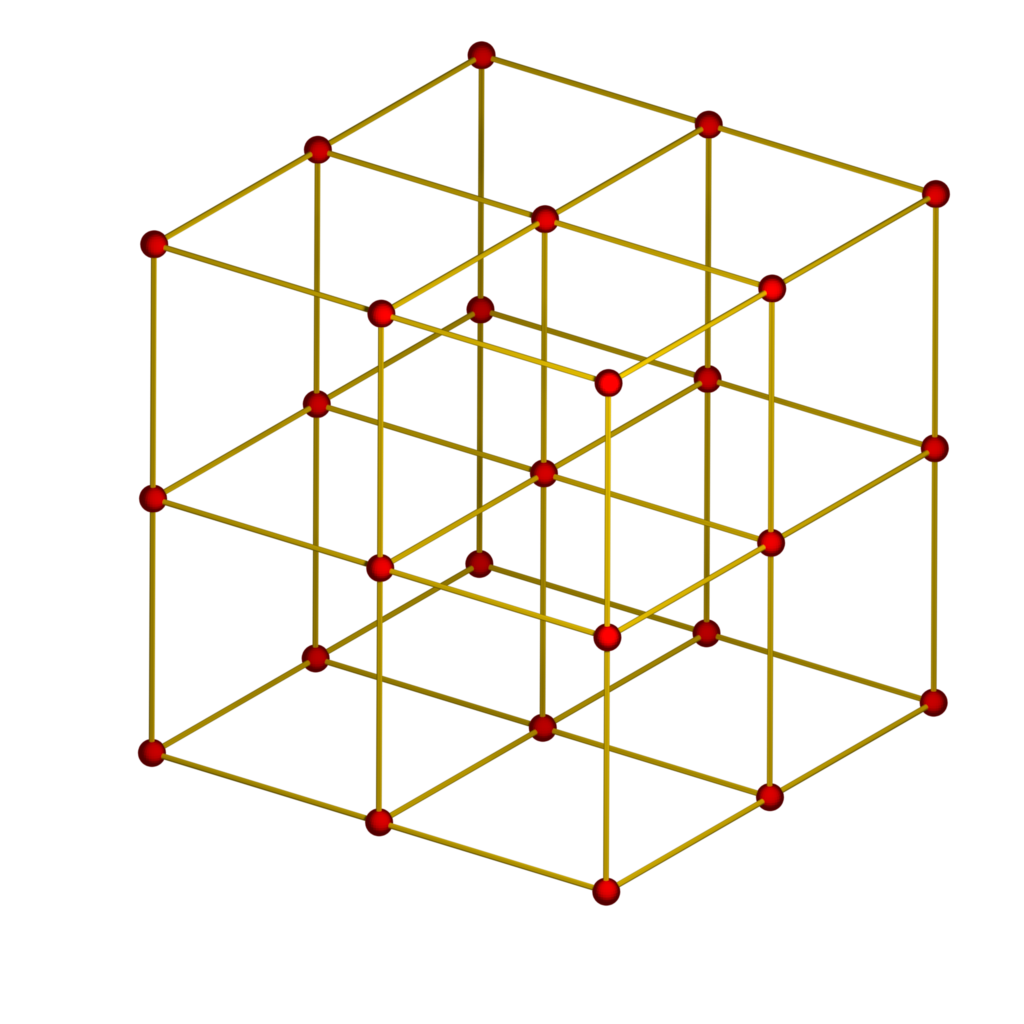
\includegraphics[width=.3\linewidth]{figures/lattice/cc}
	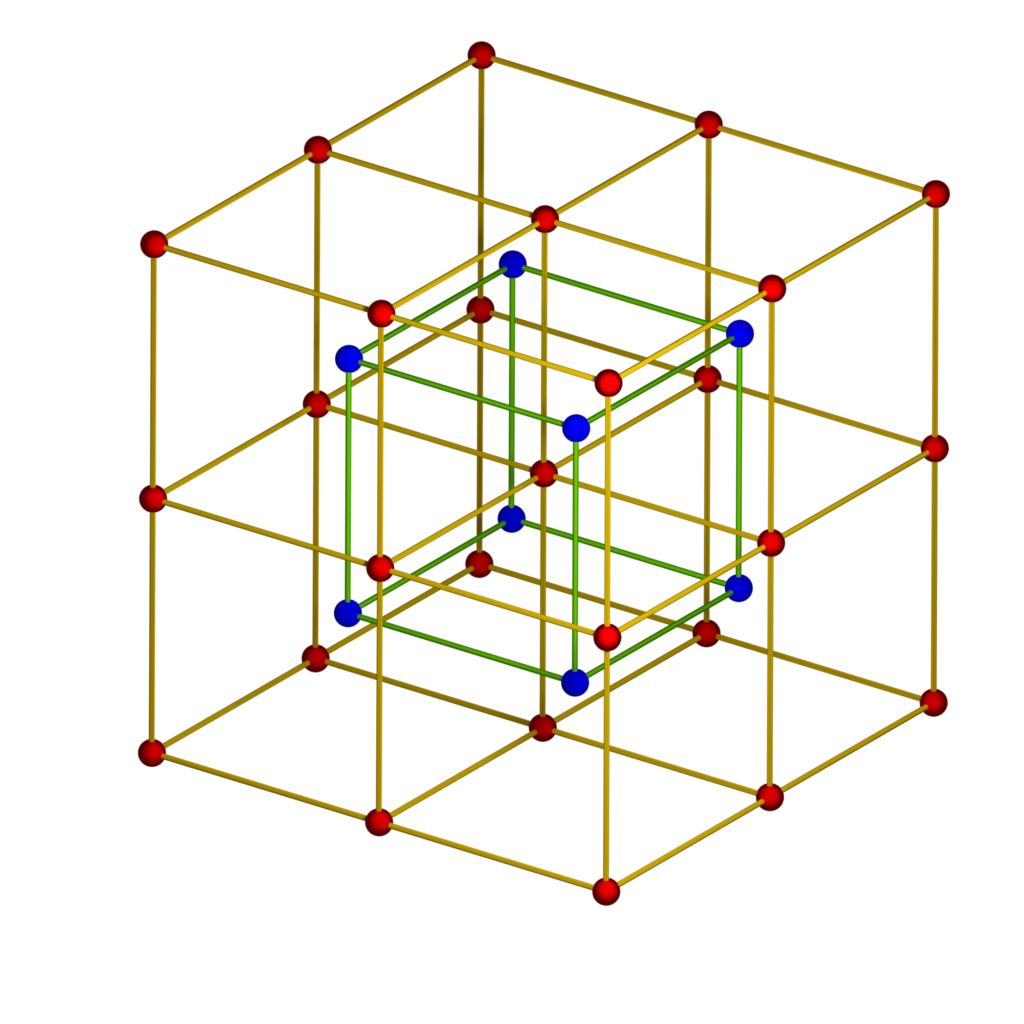
\includegraphics[width=.3\linewidth]{figures/lattice/bcc}
	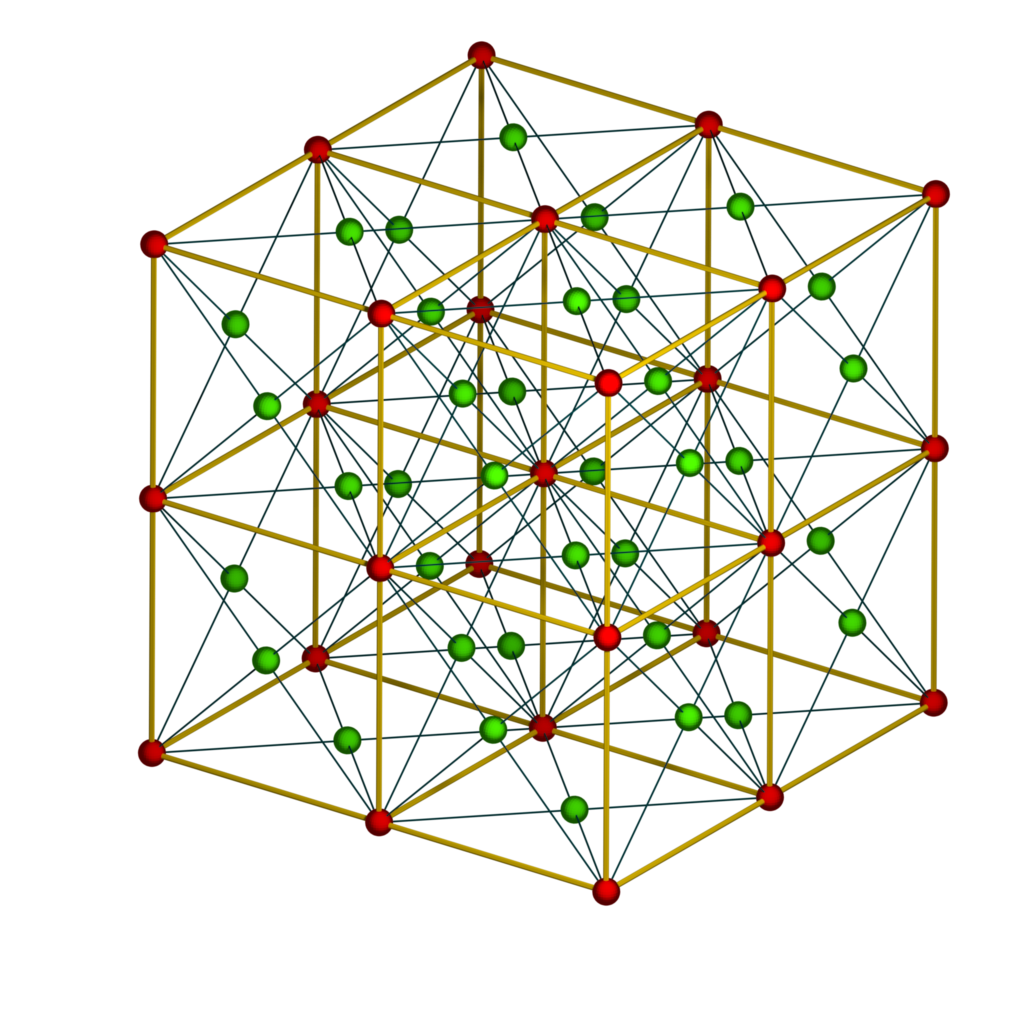
\includegraphics[width=.3\linewidth]{figures/lattice/fcc} \\
	
  \mbox{} \hfill
	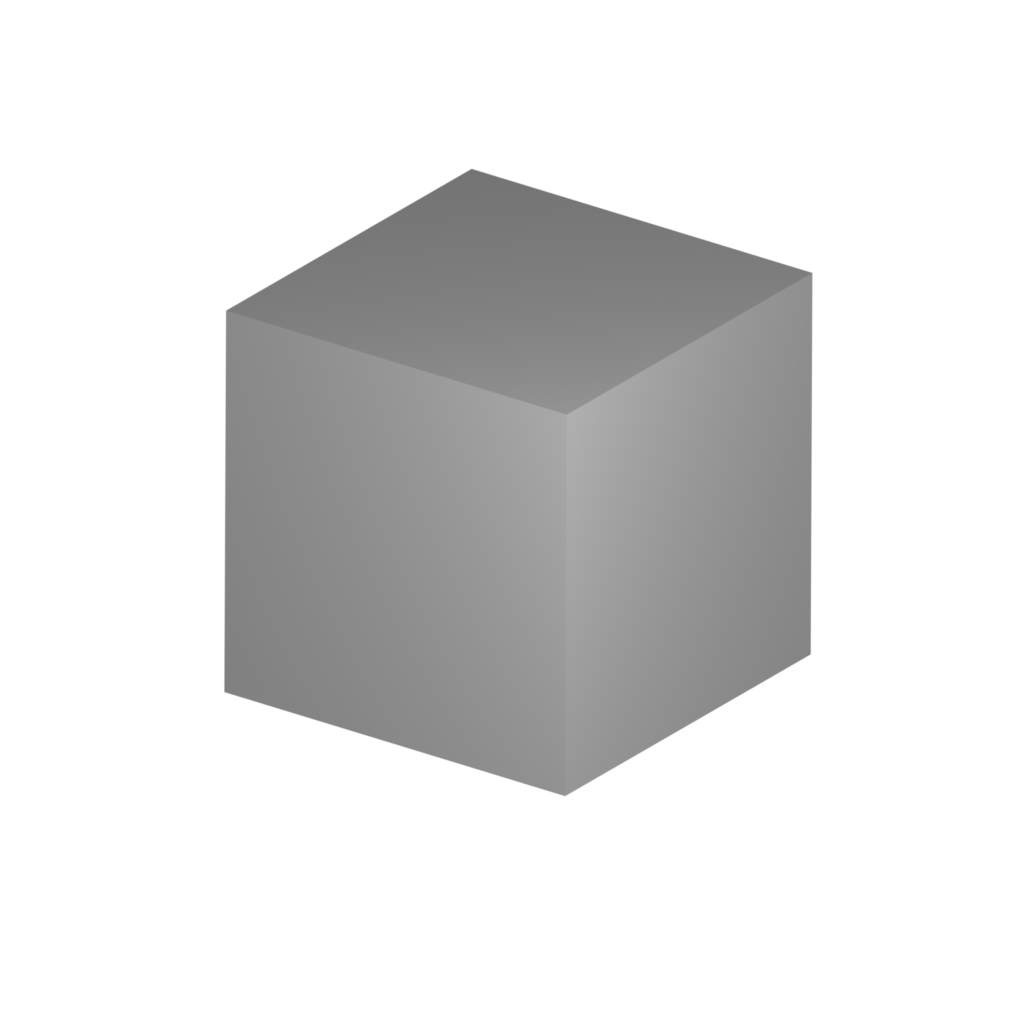
\includegraphics[width=.3\linewidth]{figures/lattice/cc_cell}
	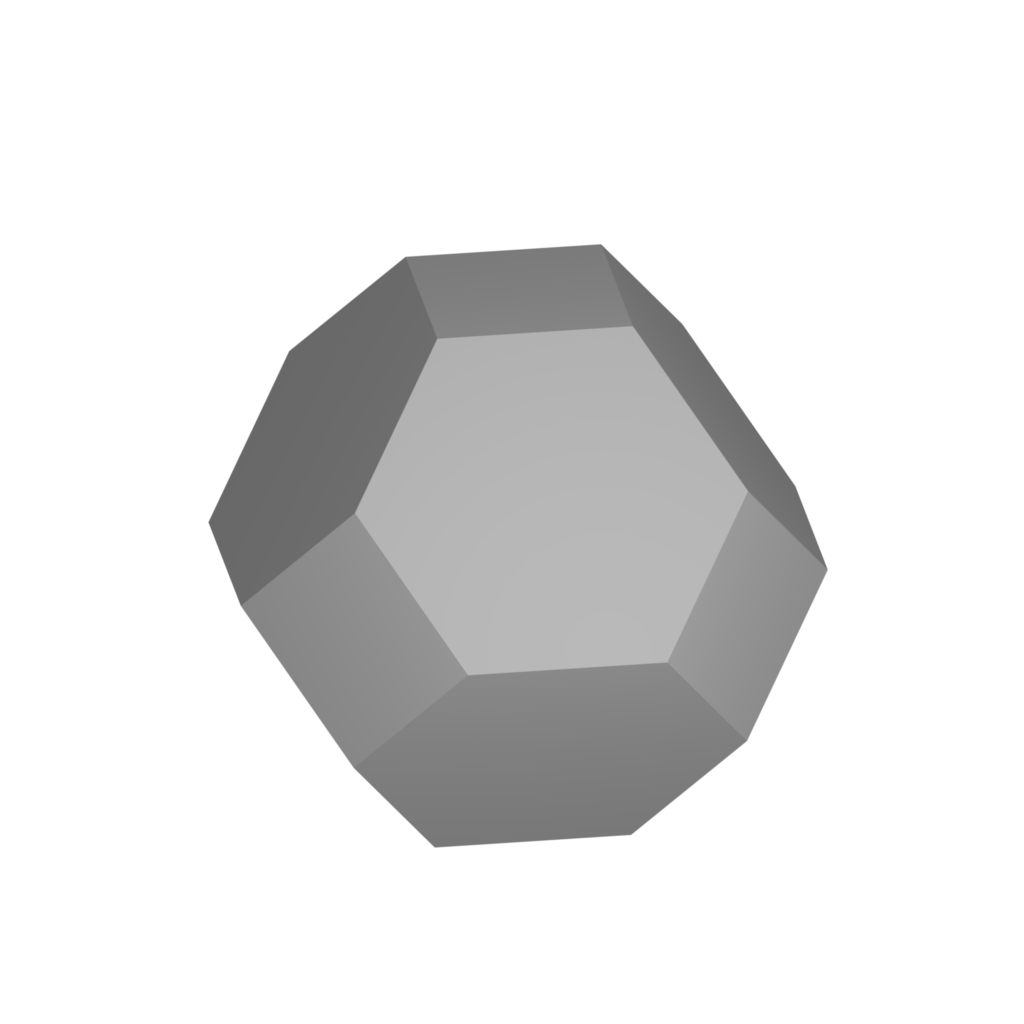
\includegraphics[width=.3\linewidth]{figures/lattice/bcc_cell}
	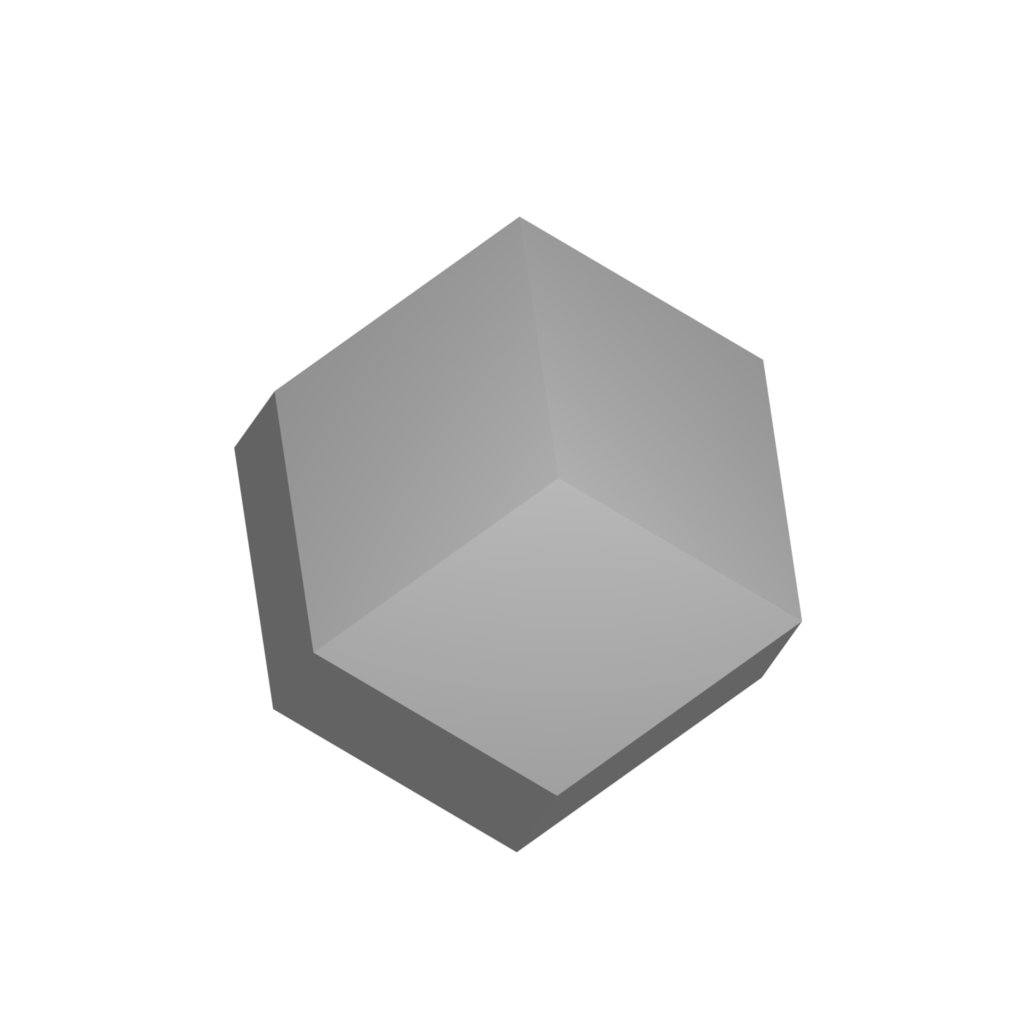
\includegraphics[width=.3\linewidth]{figures/lattice/fcc_cell} \\
   \hfill \mbox{}
  \caption{\label{fig:lattices}
  Sampling lattices (top) with with their corresponding Voronoi regions (bottom). Left to right are the CC, BCC and FCC lattices respectively.
  }
\end{figure*}

The advantage of moving to the BCC lattice is two fold. First, it's well known that the BCC lattice generates the optimal sampling pattern in $\realn^3$. The argument for optimality is simple; the sampling of a function with respect to the BCC lattice is equivalent to a periodization of it's frequency spectrum about the BCC's dual lattice, the \emph{Face Centered Cubic} (FCC) lattice. Optimality follows from the observation that the FCC lattice is the optimal sphere packing lattice in three dimensions, that is, it packs frequency replica as tightly as possible in the Fourier domain, resulting in less \emph{pre-aliasing} from sampling. For isotropically band-limited functions, this tighter packing of frequency content allows for about 30\% more information to be captured when compared to samplings generated from a Cartesian lattice. The second advantage to moving to the BCC lattice is that there exist reconstruction filters on the BCC lattice that outperform commonly used filters of equivalent order on the CC lattice in terms of both speed and accuracy \cite{practicalbox} (in software implementations) -- these filters are also more compact than their typical CC counterparts. In the context of our surface reconstruction scheme, this gives rise to regularization matrices that are more sparse on the BCC lattice and tend to provide faster convergence when optimizing the initial point set (\SC{sec:vari_review}).

Our surface reconstruction methodology follows the general Poisson approach, but with a few twists. First, we construct a smoothed approximation to the gradient field of a model's indicator function. The divergence of the gradient field is estimated and subsequently fed into a Poisson solver that outputs the coefficients needed to approximate the smoothed indicator function in a target shift invariant space. This Poisson solver is tailored to cater to the approximation power provided by each space. However, our approach is novel in two notable ways. Firstly, we employ a variational scheme to obtain a lattice-based approximation of the gradient field. This scheme depends only on the generating kernel of the target space and optimizes a functional that incorporates interpolation and smoothness constraints. Secondly, we utilize the theory behind shift-invariant spaces to seek discretizations of the divergence and Laplacian operators that are tailored to exploit the full approximation capabilities of the target space.

Additionally, we consider the possibility of approximating the smoothed gradient field representation within function spaces that are spanned by shifted versions of a single generating kernel. In the context of gradient estimation, introducing a shift in the direction of the derivative has shown to improve overall gradient approximation fidelity in terms of gradient orientation and magnitude, as well as displaying the ability to capture higher frequency details that are smoothed out in non-shifted schemes~\cite{gradrev}. Since the divergence operator is intimately connected to the gradient operator, these results are of interest to us. Using an appropriate discretization of the derivative/divergence operator is an important step in recovering the indicator function of the initial model. We also derive specific error bounds, based on an error kernel formulation, for approximations of linear operators in arbitrary shift invariant spaces.

To summarize, our contributions are as follows:
\begin{itemize}
\item[$\bullet$] We reformulate the Poisson surface reconstruction approach using general shift-invariant spaces as the target approximation space
\item[$\bullet$] Specifically, we investigate the reconstruction of surfaces in both a sub-optimal (Cartesian) and an optimal (BCC)
  box-spline function space
\item[$\bullet$] We present a new variational resampling scheme that resamples the original scattered oriented points' normals onto any regular lattice. This resampling scheme depends on the generating kernel, but is general enough to be extended to shifted generating kernels as this has been shown to improve gradient estimation in shift invariant spaces. 
\item[$\bullet$] We present an extension of the error kernel of Blu and Unser to general linear operators and show how to design filters that respect the full approximation order of the target approximation space.
\item[$\bullet$] While our focus is on comparing the surface reconstruction algorithm on both the CC and BCC lattices, we also provide qualitative and quantitative comparisons between the presented technique (on both the Cartesian and BCC lattices) and similar methods. 
\end{itemize}



\section{Related Work}
Surface reconstruction is a very active area of research in computer graphics and it's beyond the scope of this work to touch on all the material related to the subject. We therefore very briefly review some relevant contributions -- those seeking a more in-depth review may look to a recent survey of the field \cite{reconstar_eg14}.
We focus mainly on some of the more recent and related work. 

Many surface reconstruction algorithms are so-called ``\emph{implicit}'' reconstruction algorithms. 
They attempt to reconstruct an implicit function, $f : \realn^3 \mapsto \realn $, whose level-set, for some iso-value $s \in \realn$, $f(\vect{x})=s$ represents an approximation to the original surface. 
Non-implicit techniques generally infer meshes through some other combinatorial means or set predefined logic/rules.

For example, there exist many Delaunay style algorithms in which a triangulation is constructed using a subset of the original point-set \cite{delaunay}. 
The Power Crust \cite{powercrust} and Cocone \cite{cocone} algorithms are two other well-known techniques that do not construct implicit functional representations. 
These techniques often aim to exactly interpolate the input point set, and in the presence of noise tend to over-fit the surface. 
When the input data are noisy implicit approaches often perform better than non-implicit algorithms, as implicit algorithms inherently attempt to fit locally smooth basis functions to the data, averaging out any noise. 
Reconstructing either a distance function or an indicator function is common to these approaches.

One of the most well known implicit algorithms is the algorithm of by Hoppe et al.~\cite{hoppecut}. In this work a set of
tangent planes is constructed to create an approximation to a surface's distance function. 
A more recent work, is the Smoothed Signed Distance Field reconstruction technique \cite{ssdrecon}, in which an oriented point set imposes constraints on the reconstructed function, its gradient, and its Hessian. 
These constraints are equivalent to requiring that the reconstructed function be an approximation to the distance field of the original model. 
Other techniques attempt to reconstruct a signed distance function within a function space spanned by radial basis functions \cite{radial}. 
Recently, there has also been work that incorporates point normals into a radial basis reconstruction framework \cite{hermite}. 
It's also possible to construct an implicit function as a normalize sum of compactly supported basis functions defined over an oct-tree, essentially ``smearing'' the point-set around space and constructing an indicator ``shell'' around them \cite{Fuhrmann2014}.

Another implicit approach is to find an indicator function that approximates the ``inside-outside'' (indicator) function of original model. 
An early technique \cite{fftk} transforms the smoothed gradient to the Fourier domain, applies an appropriate operator, then reconstructs it in the spatial domain. 
This approach often deals well with incomplete, missing, or otherwise noisy data and has the guarantee of creating a water tight surface. 
However, it involves reconstructing the indicator on a regular grid, which becomes very memory intensive as the grid is refined.

Building on that work, Poisson surface reconstruction techniques make the observation that the Fourier method is equivalently stated as a spatial Poisson problem \cite{Kazhdan06,screenedk}. 
Moreover, they seek to rectify the memory limitations of that work, while still maintaining its benefits. However, current techniques based on this idea have been shown to over-smooth the initial point-set, and therefore the resulting surface. \cite{reconbench}.

It is also possible to reconstruct the indicator of a point set within a wavelet basis \cite{wavelet}. 
In this work, an approximate indicator function of the model is projected onto a compact wavelet basis. 
This leads to a simple and efficient algorithm even when the data sets are massive. 
However the method's speed comes at a price, as the resulting surfaces are often non-smooth, and display many ``jagged'' artefacts (although a form of smoothing is applied to the resulting indicator function in an attempt to rectify this.)

Outside of the context of surface reconstruction there has been considerable evidence that shows non-Cartesian approaches to volume rendering \cite{firstbox, practicalbox, hvolrecon} and fluid flow \cite{lboltzman} outperform Cartesian approaches in both speed and memory consumption. 
Additionally, finite difference Laplacian stencils on non-Cartesian grids lead to reduced numerical dispersion compared to their Cartesian  counterparts (see e.g. \cite{hamilton2013, hamilton2013hexagonal} and references therein). 
It is therefore natural to question whether these advantages can be exploited within the context of surface reconstruction.

Our approach aims to solve the Poisson surface reconstruction problem in the setting of general shift-invariant spaces. 
A crucial step in this regard is the accurate estimation of the divergence of the gradient field from the oriented point-set. Radial basis functions (RBFs) are generally used in the context of the reconstruction of scattered data, however, RBF techniques are often computationally expensive, requiring the solution of large unstable systems of equations (for exact interpolation). 
A proposed solution to this problem is to ``\emph{re-sample}'' the input data onto a regular shift-invariant space. 
This allows one to use efficient compact reconstruction kernels and data processing techniques \cite{variational,onvari}. 
Recently, an extension of this idea to box spline spaces \cite{xu2012rec} proposes a variational reconstruction framework in which the BCC lattice consistently outperforms the Cartesian lattice. 
Our method takes a similar variational approach and seeks to construct a smoothed lattice-based approximation of the gradient of the indicator function (\SC{sec:obtainingV}). 
Our employed constraints force the gradient to be close to zero away from the surface, while maintaining a certain degree of smoothness in the resulting approximation. 
This is preferable in comparison to other works \cite{fftk,Kazhdan06,screenedk} in which each sample is trilinearly distributed about either a grid or an oct-tree respectively, and is known to over-smooth data. 

Having obtained a high-quality lattice-based approximation of the gradient field, we invoke the theory behind shift-invariant spaces and accurately estimate the divergence by applying derivative filters that are designed to harness the full approximation capabilities of the target space (\SC{sec:divergence}). 

Once the smoothed gradient's divergence has been calculated, recovering the indicator function is a simple matter of taking the inverse of the Laplacian over domain (i.e. solving the Poisson system). 
To do this, we take an approach that is also inspired by filtering methodologies in signal processing. In particular, we're interested in an approximate solution to Poisson?s equation that lies in a chosen shift-invariant space. 
Our solution methodology is reminiscent of the finite element method. However, we do not impose any boundary conditions on the generating kernels. Rather, we satisfy homogeneous Dirichlet boundary conditions implicitly by requiring that the coefficient sequence be odd (Section III). 
The solution is obtained by applying a digital filter to point samples. We approach the problem from first principles and derive the tools necessary to design solution filters for a chosen shift-invariant space (\SC{sec:recoveringX}).

%\section{Preliminaries}\label{sec:pois_review}
\subsection{Poisson Surface Reconstruction}
We denote the indicator function of a model $M$ as $$ \chi_M(\mathbf{x}) :=
\begin{cases}
1, & \text{if }\mathbf{x}\text{ is in the interior of the model } M \\
\frac{1}{2}, & \text{if } \mathbf{x}\text{ is on the model's surface}\\
0, & \text{if }\mathbf{x}\text{ is exterior to } M
\end{cases}. $$
Integral to formulating surface reconstruction as a Poisson problem, is the observation that if one obtains some function $\vec{V}(\mathbf{x})\approx{\nabla}\chi_M$ that approximates the smoothed gradient of the indicator function, finding an approximation to the indicator function reduces to finding a $\inda$ such that {\small 
\begin{equation} \label{eq:poisson}
	\lapl{\inda} = {\grad} \cdot \vec{V}.
\end{equation}}
We define the set of input surface points to be $P:=\{(\mathbf{p}_1,\mathbf{n}_1), (\mathbf{p}_2,\mathbf{n}_2) \hdots (\mathbf{p}_M,\mathbf{n}_M) : (\mathbf{p}_i,\mathbf{n}_i) \in
\realn^3 \times \realn^3 \}$ where $\mathbf{p}_i$ and $\mathbf{n}_i$ are the position and normal vector of the $i^{th}$ sample respectively. Orientation can be succinctly represented with only two values, however, it is convenient to keep it denoted as the normal at a point. This is because the length of the normal can be used to encode the sampling density of the point-set at a point. For the following discussion, we also need to introduce the notation $\patch_{\mathbf{s}}$, which denotes a patch of the surface model about the sample location $\mathbf{s}$. 

Inspired by the approach of Kazhdan et al.~\cite{Kazhdan06} the approximation $\vec{V}(\vx)$ is defined to be  {\small 
\begin{eqnarray}
	\vec{V}(\vx) & := & \sum_{(\mathbf{s},\mathbf{n}) \in P}\left|\patch_s\right|F(\vx-\mathbf{s})\cdot\vn \label{eq:vdef} \\
	 & \approx & \sum_{(\mathbf{s},\mathbf{n}) \in P} \int_{\patch_s}{F(\mathbf{x} - \mathbf{p}) \nabla \chi (\mathbf{p})} \mathrm{d} \mathbf{p}. \notag  
\end{eqnarray}}
Thus, $\vec{V}(\vx)$ approximates the gradient of the indicator smoothed by some filter $F$, broken up over surface patches of the model. We assume the point sampling to be uniform, thus the area of each patch $\left|\patch_s\right|$ should be a constant, and our resulting approximation will be scaled by an unknown factor. We return to this in \SC{sec:levelset}. The choice of $F$ places computational constraints on the resulting algorithm.

$F$ is often explicitly chosen to be a compactly supported function. This simplifies and reduces the computational cost of the method when used in conjunction with an oct-tree based representation of $\vec{V}(\vx)$ \cite{Kazhdan06}. However, there is a disadvantage in that $F$ may over smooth data in areas of high curvature \cite{reconbench}, much in the same way that a representation of a sampled signal may fail to take advantage of the full approximation power of the function space in which it is represented if it is not properly prefiltered. Theoretically, one could reconstruct the surface at higher resolutions, allowing the basis functions to become more ``fine'', but increasing the total amount of memory used. However, this is not realistic in praxis. Another approach is to impose a type of ``interpolation'' constraint on the original data \cite{screenedk}.

Ideally, the filter $F$ should correspond to some globally supported RBF. However, as the support of $F$ grows, so does the cost of evaluating it at lattice sites. Moreover, the added benefit of a globally supported RBF is partially lost as the subsequent steps are entirely lattice-based and do not take the RBF into consideration. Our approach circumvents the choice of $F$ entirely by posing the gradient approximation problem as a variational problem that, in addition to imposing the interpolation constraint, also imposes constraints on the ``compactness'' and ``smoothness'' of the gradient approximation. The only kernel we need to consider is the one that generates our target shift-invariant space, i.e. the space used to recover the smoothed indicator function. This type of variational reconstruction can be seen as an approximation to radial basis approaches~\cite{variational}, and is well-suited to our Poisson formulation in shift-invariant spaces.

Before presenting our approach (\SC{sec:pipeline}), we review the necessary background behind shift-invariant spaces and its connection to irregular sampling.
%\ednote{UA: Provided additional motivation for the variational framework, and added a gluing paragraph to imrpove the flow.}

\subsection{Sampling Lattices} \label{sec:smpl_review}
In the univariate case, there is only one way to uniformly sample a signal; take equally spaced samples along the independent axis. However, when sampling multivariate signals, the situation is not as straightforward. A common approach is to inherit the ideas from the univariate case, and sample the function at regular intervals in each axis (known as a Cartesian sampling), while another might be to place samples at the centres of spheres arranged in the densest possible sphere packing (otherwise known as an FCC sampling). If $\mathbf{L}$ is a unimodular matrix, the set $\{\mathbf{L}\cdot\mathbf{n} : \mathbf{n} \in \intn^3 \}$ (linear combinations of the vectors of $\mathbb{L}$ with integer coefficients), represents all possible sampling lattices. $\mathbf{L}$ is often called the \emph{generating matrix} for a lattice. To control the sampling rate of a function, a uniform scaling parameter $h$ is introduced. Typically, for the problem of surface reconstruction, our input data are not uniformly distributed in space (or even about the surface of the model). However, the concept of a sampling lattice is fundamental in forming the definition of our target approximation spaces (\SC{sec:sis_review}).

The Cartesian lattice is given by the generating matrix $\mathbf{L}_C:=\mathbf{I}_3$, where $\mathbf{I}_3$ is the $3 \times 3$ identity matrix. There are many factors that contribute to the ubiquity of the Cartesian lattice in practice. Possibly one of its most attractive features is its separability. Owing to this, the implementation of generating functions that span function spaces on the Cartesian lattice may be realized by a tensor product extension of existing univariate techniques. Filtering techniques are also easy to implement, as the Fast Fourier Transform is also separable, and may be applied independently to each axis of the data. However, in terms of sampling efficiency, the BCC lattice is the optimal lattice in $\realn^3$, while the Cartesian is sub-optimal.

The Body-Centered Cubic (BCC) lattice is generated by the integer matrix  {\footnotesize
\begin{equation*} 
	\mathbf{L}_B := 
	\begin{bmatrix}
		-1 & 1 & 1 \\ 
		1 & -1 & 1 \\ 
		1 & 1 & -1 
	\end{bmatrix}.
\end{equation*}}
However, the BCC lattice is non-separable, and requires special care in data retrieval and indexing. \FG{fig:lattices} shows these lattices and their Voronoi regions, including the dual of the BCC lattice, the FCC lattice (the Cartesian lattice is dual to itself.)

\subsection{Box Splines}
\label{sec:box_review}
Box splines are compact piece-wise polynomial functions $ M_\mathbf{\Xii} : \realn^s \to \realn.$ The matrix $\mathbf{\Xii}$ denotes a collection of direction vectors, $\mathbf{\Xii} := \left[ \xi_1 \ \xi_2 \hdots \xi_n\right].$ When $n=s$, the function $M_\mathbf{\Xii}(\vx)$ is defined to be $\frac{1}{det|\mathbf{\Xii}|}$ inside the polytope formed by the Minkowski sum of the direction vectors of $\mathbf{\Xii}$, and zero otherwise (that is, $\frac{1}{det|\mathbf{\Xii}|}$ when $\vx \in \{ \mathbf{\xi}_1 t_1 + \hdots + \mathbf{\xi}_s t_s  : t_i\in [0,1) \})$. When $n > s$, the box spline is recursively defined as {\small 
\begin{equation} \label{eq:box_def}
	M_{\mathbf{\Xii}}(\vx) := \int_0^1{\!M_{\mathbf{\Xii/\xi}_n}(\vx - t\mathbf{\xi}_n)} \mathrm{d}t,
\end{equation}}
where $\!M_{\mathbf{\Xii/\xi}_n}$ is the matrix obtained by removing the column vector $\xi_n$ from $\mathbf{\Xii}$. Box splines are a natural fit for our purposes, and are chosen to span our function spaces. One motivating factor that encourages the use of box splines on the BCC lattice over the Cartesian lattice is that the support of the box splines on the BCC lattice contains less lattice sites as opposed to their Cartesian counterparts. At the same time, they maintain the same order of accuracy and smoothness. This implies that one should expect roughly the same quality reconstruction, with less memory accesses per reconstructed value.

The evaluation of a box spline, in general, can be achieved by evaluating a simple recursive expression \cite{boorboxsplines}. However, for many purposes, this form of evaluation is too slow. There has been a line of research \cite{firstbox} aimed towards obtaining fast piecewise polynomial representations of the box splines on the BCC lattice, and showing their advantage in speed and accuracy over splines on the Cartesian lattice when the data to be interpolated are sufficiently smooth.

\begin{figure}
  \centering
  \mbox{} \hfill
	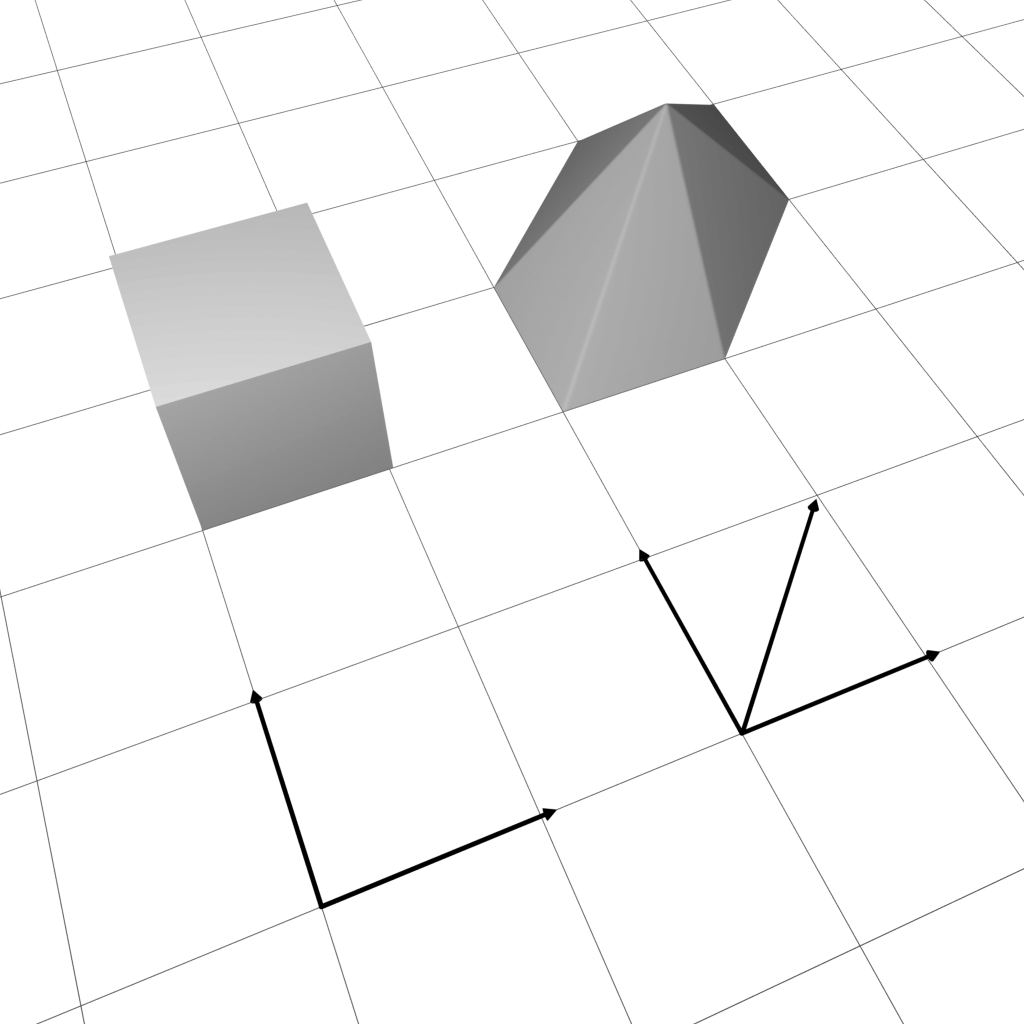
\includegraphics[width=\linewidth]{figures/boxspline/2dex}
  \caption{\label{fig:box2d}%
  An example of box splines in 2D. On the left is the box spline comprised of the direction vectors $\mathbf{\xi}_1, \mathbf{\xi}_2$, (the case n=s) which is the indicator function of the Minkowski sum of the vectors. The box spline on the right, includes a third vector $\mathbf{\xi}_3$, which can be thought of as ``smearing'' the first spline along the direction $\mathbf{\xi}_3$.
  }
\end{figure}


\subsubsection{Cartesian Lattice}
Choosing $\mathbf{\Xii = \Xii_{C2} := \left[ I_3  \ I_3 \right]}$ (the $3 \times 6$ matrix created by the union of two identity matrices) generates a triliniear piecewise polynomial. It is easy to see, by definition, when $\mathbf{\Xii_{C2}}$ is used in conjunction with \EQp{eq:box_def}, the resulting function $M_\mathbf{\Xii_{C2}}(\vx)$ corresponds to the non-centered tensor product extension of the linear B-spline in three dimensions. Likewise, the non-centered cubic tensor product box spline is given by $M_\mathbf{\Xii_{C4}}(\vx)$, where $\mathbf{\Xii_{C4} := \left[ I_3  \ I_3 \ I_3  \ I_3 \right]}$. A box spline is easily centered by taking $M_\mathbf{\Xii}(\vx + \mathbf{c_\Xii})$, with $\mathbf{c_\Xii}:=\sum_{\xi \in \mathbf{\Xii}} \frac{1}{2}\xi$. We will assume, unless otherwise stated, that $M_\mathbf{\Xii}$ defines the centered box spline generated by $\mathbf{\Xii}$.

\subsubsection{BCC Lattice}
On the BCC lattice, a choice of {\footnotesize
\begin{equation*}
	\mathbf{\Xii_{B}} := 
	\begin{bmatrix} 
		-1 & 1 & 1 & -1 \\
		1 & -1 & 1 & -1 \\
		1 & 1 & -1 & -1 
	\end{bmatrix}
\end{equation*}}
generates a piecewise linear polynomial function \cite{practicalbox}. The support of this box spline is a rhombic dodecahedron, which incidentally contains the set of first nearest neighbors to the Voronoi region of the lattice at the origin, and is a natural fit for the lattice. The quintic box spline is given by the matrix $\mathbf{\Xii_{B2}} := \left[\mathbf{\Xii_{B}} \ \mathbf{\Xii_{B}}\right]$, or may also be seen as the convolution of the linear box spline with itself.  However, there exist both an efficient piecewise polynomial representation \cite{practicalbox}, and an efficient implementation \cite{fastbox} of these piecewise quintic polynomial functions.

\subsubsection{Shifted Basis Functions}
We also consider shifted box splines $M_{\mathbf{\Xii}}^{\xi_i}(\vx) := M_{\mathbf{\Xii}}(\vx - \frac{1}{2}\mathbf{\xi}_i)$, where $\mathbf{\xi}_i$ is any direction vector in $\mathbf{\Xii}$. In the univariate case with linear B-splines, it has been shown that introducing a shift can offer an improvement when representing scalar data \cite{linearrev}. More generally and relevant to our purposes, they have also been shown to reduce error when approximating the gradient of scalar fields \cite{gradrev}.

\subsection{Shift Invariant Spaces} \label{sec:sis_review}
As our target reconstruction spaces, we consider the shift-invariant spaces defined by {\small 
\begin{equation*}
	\fspce{\varphi}{h\mathbf{L}} := \left\{ g(\vx) := \displaystyle\sum_{\mathbf{m} \in \intn^3} c[\mathbf{m}]\genfuncdef{\vx} : c \in \ell_2 \right\},
\end{equation*}}
where $\varphi$ is the generating function for the space, $h$ is a scaling parameter that controls the sampling rate or granularity, and $\mathbf{L}$ is the generating matrix for a given sampling lattice. Representing a function $f$ in a shift invariant space boils down to finding an appropriate coefficient $c[\mathbf{m}]$ vector that brings $g$ as close as possible to the true underlying function $f$. 

If the generating function that spans the space satisfies the \emph{Strang-Fix} conditions of order $k$, and $f$ belongs to the Sobolev space of at least order $k$, then it can be shown that the minimum approximation error (in the least-squares sense) decays asymptotically as $O(h^k)$, and the space is said to have approximation order $k$. We often only have access to $f$ through a discrete amount of samples, $\mathbf{f} := \left[ f_1 \ f_2 \ \hdots \ f_M \right]^T$ located at sample points $S := \{\vx_1, \vx_2 \hdots \vx_M \}$ respectively. When this is the case, the minimum-error approximation is unattainable. However, interpolative and quasi-interpolative methods \cite{quasibcc,interprev}, which can be seen as oblique projections onto $\fspce{\varphi}{h\mathbf{L}}$, maintain the same order of accuracy.

For sufficiently smooth functions $f$ that are uniformly sampled and properly prefiltered, the trilinear and linear reconstruction filters (Cartesian and BCC respectively) assure second order convergence, while the tricubic and Quintic assure fourth order. Another nicety of these spaces is that data processing techniques --- derivative approximation for example --- can often be represented by a convolution of the coefficient vector with either an \emph{Infinite Impulse Response} (IIR) or \emph{Finite Impulse Response} (FIR) filter. 

Typically, as memory is a limited quantity, we are only interested in a finite number of points on a lattice. We denote the set of such points as $\{\mathbf{s}_1,\mathbf{s}_2,\ \hdots  \ \mathbf{s}_N\} \subset \mathbf{L}\intn^3.$ Corresponding to each lattice site is a coefficient $c_k$; we collect all such coefficients in the column vector $\mathbf{c}:=\left[c_1 \ c_2 \ \hdots \ c_N \right]^T.$ We also use the short hand notation $\varphi_k(\vx) := \varphi(\frac{\vx}{h}-\mathbf{s}_k)$; from this perspective, our function space is now {\small 
\begin{equation}
	\left\{ \displaystyle\sum_{k=0}^N c_k \varphi_k(\vx) \right\} \subset \fspce{\varphi}{h\mathbf{L}}.
\end{equation}}
Further, we denote $\mathbf{\Phii}$ to be the $M \times N$ matrix whose elements are given by sampling the basis functions anchored at each lattice site, or $\Phii_{i,j} := \varphi_j(\vx_i)$. Clearly, if our data are sampled at the lattice sites ($\vx_i = \mathbf{s}_i$), then the problem of finding an interpolative scheme reduces to finding $\mathbf{c}$ such that $\mathbf{\Phii c=f},$ which only involves inverting the square matrix $\mathbf{\Phii}.$ However, our sample locations are almost certain to not coincide with lattice sites, and we must consider alternative schemes for finding $\mathbf{c}.$

\subsection{Irregular Sampling}
\label{sec:vari_review}
%When reconstructing functions whose data are sampled regularly on a lattice, finding an oblique projection of the original function in the target function space is relatively straight-forward. However, except on very rare occasions, samples placed over the surface of a model do not coincide with lattice sites. A solution to this problem is to ``re-sample'' the input point set onto said lattices sites.
In the work by Kazdhan et al. \cite{fftk} the range data are splatted via a linear filter onto a regular Cartesian grid. This tends to over-smooth the resulting reconstruction, as it allows the surface to deviate from the original sample locations. Ideally, we would like to find a function that not only interpolates the input data, but provides the representation with the smallest possible ``shell'' about the initial point set (i.e., the fewest non zero coefficients) while still interpolating the data and eliciting a unique solution. 

Thus, we recast the problem of finding a representation of $g$ within our function space as an optimization problem. There are similar works that impose variational constraints on random point samples for images \cite{variational}, as well as multi-resolution techniques for volumetric data \cite{onvari} and an extension to box spline spaces \cite{xu2012rec}. In the same vein, we seek a function $g \in \fspce{\varphi}{h\mathbf{L}}$ that attempts to interpolate the input data, and minimize a functional $E$. Specifically, we seek a $g$ that minimizes {\small 
\begin{equation} \label{eq:minexp}
 	\sump_{i=1}^{M} (g(\vx_i) -  f_i)^2 + E(g).
\end{equation}}
It is important to introduce a bit of notation before proceeding, $\dv{\mathbf{v}} f := \mathbf{v} \cdot \grad f$ defines the directional derivative of $f$ in the direction $\mathbf{v}$. The Beppo-Levi inner product of order $n$ is defined as $\blip{n}{f}{g}:= \sum_{|\mathbf{p}|=n}({n!}/{\mathbf{p}!}) \innerp{\mathbf{D^p}f}{\mathbf{D^p}g}$, where $\mathbf{p}$ is an integer vector such that $\left| \mathbf{p}\right| := p_1 + p_2 + p_3 $. We also use the short hand $\mathbf{D^p}f := \partial^{\left| \mathbf{p}\right|}f/({\partial^{p_1}x_1}{\partial^{p_2}x_2}{\partial^{p_3}x_3}).$ The second order Beppo-Levi norm of $f$ is defined as $\bln{2}{f}^2:=\blip{2}{f}{f}$.

The second order Beppo-Levi norm can be thought to measure the ``smoothness'' of a function. However, constraining the smoothness of our approximation alone is not sufficient to elicit the desired solution in our case. We propose that the smoothed normal field should also minimize the inner product of the function with itself. This has the physical interpretation of forcing the solution to be close to zero everywhere except near the input points. Our proposed cost functional is then $E(g) := \lambda_1 \left|\left|{g}\right|\right| + \lambda_2 \bln{2}{g}.$ Here, $\lambda_1$ controls the amount to which the function is penalized for large coefficient values. When combined with the interpolation constraint, this imposes the behavior of forcing the function to be zero away from the surface. The parameter $\lambda_2$ controls the smoothness of the resulting normal field.
%\begin{equation} \label{eq:functional}
%	E(g) := \lambda_1 \left|\left|{g}\right|\right| + \lambda_2 \bln{2}{g}.
%\end{equation}

Finding $g$ that minimizes equation \EQ{eq:minexp} involves rewriting the minimization problem in terms of $\mathbf{c}$ \cite{xu2012rec}. Following some straightforward algebraic manipulations (see \cite{xu2012rec} for details), the coefficient vector can be obtained by taking $\mathbf{c} = ( \mathbf{\Phii}^T\mathbf{\Phii} + \lambda_1\mathbf{G} + \lambda_2\mathbf{S})^{-1}\mathbf{\Phii}^T\mathbf{f}$, where $G_{i,j}:=\innerp{\varphi_i}{\varphi_j}$ and $S_{i,j}:=\blip{2}{\varphi_i}{\varphi_j}$. Since $\varphi$ is known in closed form, the entries of both $\mathbf{G}$ and $\mathbf{S}$ can be evaluated analytically. The above vector equation can be efficiently solved using the Conjugate Gradient method.
%\begin{equation}
%	\mathbf{c} = \left( \mathbf{\Phii}^T\mathbf{\Phii} + \lambda_1\mathbf{G} + \lambda_2\mathbf{S}\right)^{-1}\mathbf{\Phii}^T\mathbf{f},
%\label{eq:variationalSolution}
%\end{equation}
\section{Preliminaries}\label{sec:pois_review}
\subsection{Poisson Surface Reconstruction}
We denote the indicator function of a model $M$ as $$ \chi_M(\mathbf{x}) :=
\begin{cases}
1, & \text{if }\mathbf{x}\text{ is in the interior of the model } M \\
\frac{1}{2}, & \text{if } \mathbf{x}\text{ is on the model's surface}\\
0, & \text{if }\mathbf{x}\text{ is exterior to } M
\end{cases}. $$
Integral to formulating surface reconstruction as a Poisson problem, is the observation that if one obtains some function $\vec{V}(\mathbf{x})\approx{\nabla}\chi_M$ that approximates the smoothed gradient of the indicator function, finding an approximation to the indicator function reduces to finding a $\inda$ such that {\small 
\begin{equation} \label{eq:poisson}
	\lapl{\inda} = {\grad} \cdot \vec{V}.
\end{equation}}
We define the set of input surface points to be $P:=\{(\mathbf{p}_1,\mathbf{n}_1), (\mathbf{p}_2,\mathbf{n}_2) \hdots (\mathbf{p}_M,\mathbf{n}_M) : (\mathbf{p}_i,\mathbf{n}_i) \in
\realn^3 \times \realn^3 \}$ where $\mathbf{p}_i$ and $\mathbf{n}_i$ are the position and normal vector of the $i^{th}$ sample respectively. Orientation can be succinctly represented with only two values, however, it is convenient to keep it denoted as the normal at a point. This is because the length of the normal can be used to encode the sampling density of the point-set at a point. For the following discussion, we also need to introduce the notation $\patch_{\mathbf{s}}$, which denotes a patch of the surface model about the sample location $\mathbf{s}$. 

Inspired by the approach of Kazhdan et al.~\cite{Kazhdan06} the approximation $\vec{V}(\vx)$ is defined to be  {\small 
\begin{eqnarray}
	\vec{V}(\vx) & := & \sum_{(\mathbf{s},\mathbf{n}) \in P}\left|\patch_s\right|F(\vx-\mathbf{s})\cdot\vn \label{eq:vdef} \\
	 & \approx & \sum_{(\mathbf{s},\mathbf{n}) \in P} \int_{\patch_s}{F(\mathbf{x} - \mathbf{p}) \nabla \chi (\mathbf{p})} \mathrm{d} \mathbf{p}. \notag  
\end{eqnarray}}
Thus, $\vec{V}(\vx)$ approximates the gradient of the indicator smoothed by some filter $F$, broken up over surface patches of the model. We assume the point sampling to be uniform, thus the area of each patch $\left|\patch_s\right|$ should be a constant, and our resulting approximation will be scaled by an unknown factor. We return to this in \SC{sec:levelset}. The choice of $F$ places computational constraints on the resulting algorithm.

$F$ is often explicitly chosen to be a compactly supported function. This simplifies and reduces the computational cost of the method when used in conjunction with an oct-tree based representation of $\vec{V}(\vx)$ \cite{Kazhdan06}. However, there is a disadvantage in that $F$ may over smooth data in areas of high curvature \cite{reconbench}, much in the same way that a representation of a sampled signal may fail to take advantage of the full approximation power of the function space in which it is represented if it is not properly prefiltered. Theoretically, one could reconstruct the surface at higher resolutions, allowing the basis functions to become more ``fine'', but increasing the total amount of memory used. However, this is not realistic in praxis. Another approach is to impose a type of ``interpolation'' constraint on the original data \cite{screenedk}.

Ideally, the filter $F$ should correspond to some globally supported RBF. However, as the support of $F$ grows, so does the cost of evaluating it at lattice sites. Moreover, the added benefit of a globally supported RBF is partially lost as the subsequent steps are entirely lattice-based and do not take the RBF into consideration. Our approach circumvents the choice of $F$ entirely by posing the gradient approximation problem as a variational problem that, in addition to imposing the interpolation constraint, also imposes constraints on the ``compactness'' and ``smoothness'' of the gradient approximation. The only kernel we need to consider is the one that generates our target shift-invariant space, i.e. the space used to recover the smoothed indicator function. This type of variational reconstruction can be seen as an approximation to radial basis approaches~\cite{variational}, and is well-suited to our Poisson formulation in shift-invariant spaces.

Before presenting our approach (\SC{sec:pipeline}), we review the necessary background behind shift-invariant spaces and its connection to irregular sampling.
%\ednote{UA: Provided additional motivation for the variational framework, and added a gluing paragraph to imrpove the flow.}

\subsection{Sampling Lattices} \label{sec:smpl_review}
In the univariate case, there is only one way to uniformly sample a signal; take equally spaced samples along the independent axis. However, when sampling multivariate signals, the situation is not as straightforward. A common approach is to inherit the ideas from the univariate case, and sample the function at regular intervals in each axis (known as a Cartesian sampling), while another might be to place samples at the centres of spheres arranged in the densest possible sphere packing (otherwise known as an FCC sampling). If $\mathbf{L}$ is a unimodular matrix, the set $\{\mathbf{L}\cdot\mathbf{n} : \mathbf{n} \in \intn^3 \}$ (linear combinations of the vectors of $\mathbb{L}$ with integer coefficients), represents all possible sampling lattices. $\mathbf{L}$ is often called the \emph{generating matrix} for a lattice. To control the sampling rate of a function, a uniform scaling parameter $h$ is introduced. Typically, for the problem of surface reconstruction, our input data are not uniformly distributed in space (or even about the surface of the model). However, the concept of a sampling lattice is fundamental in forming the definition of our target approximation spaces (\SC{sec:sis_review}).

The Cartesian lattice is given by the generating matrix $\mathbf{L}_C:=\mathbf{I}_3$, where $\mathbf{I}_3$ is the $3 \times 3$ identity matrix. There are many factors that contribute to the ubiquity of the Cartesian lattice in practice. Possibly one of its most attractive features is its separability. Owing to this, the implementation of generating functions that span function spaces on the Cartesian lattice may be realized by a tensor product extension of existing univariate techniques. Filtering techniques are also easy to implement, as the Fast Fourier Transform is also separable, and may be applied independently to each axis of the data. However, in terms of sampling efficiency, the BCC lattice is the optimal lattice in $\realn^3$, while the Cartesian is sub-optimal.

The Body-Centered Cubic (BCC) lattice is generated by the integer matrix  {\footnotesize
\begin{equation*} 
	\mathbf{L}_B := 
	\begin{bmatrix}
		-1 & 1 & 1 \\ 
		1 & -1 & 1 \\ 
		1 & 1 & -1 
	\end{bmatrix}.
\end{equation*}}
However, the BCC lattice is non-separable, and requires special care in data retrieval and indexing. \FG{fig:lattices} shows these lattices and their Voronoi regions, including the dual of the BCC lattice, the FCC lattice (the Cartesian lattice is dual to itself.)

\subsection{Shift Invariant Spaces} \label{sec:sis_review}
As our target reconstruction spaces, we consider the shift-invariant spaces defined by {\small 
\begin{equation*}
	\fspce{\varphi}{h\mathbf{L}} := \left\{ g(\vx) := \displaystyle\sum_{\mathbf{m} \in \intn^3} c[\mathbf{m}]\genfuncdef{\vx} : c \in \ell_2 \right\},
\end{equation*}}
where $\varphi$ is the generating function for the space, $h$ is a scaling parameter that controls the sampling rate or granularity, and $\mathbf{L}$ is the generating matrix for a given sampling lattice. Representing a function $f$ in a shift invariant space boils down to finding an appropriate coefficient $c[\mathbf{m}]$ vector that brings $g$ as close as possible to the true underlying function $f$. 

If the generating function that spans the space satisfies the \emph{Strang-Fix} conditions of order $k$, and $f$ belongs to the Sobolev space of at least order $k$, then it can be shown that the minimum approximation error (in the least-squares sense) decays asymptotically as $O(h^k)$, and the space is said to have approximation order $k$. We often only have access to $f$ through a discrete amount of samples, $\mathbf{f} := \left[ f_1 \ f_2 \ \hdots \ f_M \right]^T$ located at sample points $S := \{\vx_1, \vx_2 \hdots \vx_M \}$ respectively. When this is the case, the minimum-error approximation is unattainable. However, interpolative and quasi-interpolative methods \cite{quasibcc,interprev}, which can be seen as oblique projections onto $\fspce{\varphi}{h\mathbf{L}}$, maintain the same order of accuracy.

For sufficiently smooth functions $f$ that are uniformly sampled and properly prefiltered, the trilinear and linear reconstruction filters (Cartesian and BCC respectively) assure second order convergence, while the tricubic and Quintic assure fourth order. Another nicety of these spaces is that data processing techniques --- derivative approximation for example --- can often be represented by a convolution of the coefficient vector with either an \emph{Infinite Impulse Response} (IIR) or \emph{Finite Impulse Response} (FIR) filter. 

Typically, as memory is a limited quantity, we are only interested in a finite number of points on a lattice. We denote the set of such points as $\{\mathbf{s}_1,\mathbf{s}_2,\ \hdots  \ \mathbf{s}_N\} \subset \mathbf{L}\intn^3.$ Corresponding to each lattice site is a coefficient $c_k$; we collect all such coefficients in the column vector $\mathbf{c}:=\left[c_1 \ c_2 \ \hdots \ c_N \right]^T.$ We also use the short hand notation $\varphi_k(\vx) := \varphi(\frac{\vx}{h}-\mathbf{s}_k)$; from this perspective, our function space is now {\small 
\begin{equation}
	\left\{ \displaystyle\sum_{k=0}^N c_k \varphi_k(\vx) \right\} \subset \fspce{\varphi}{h\mathbf{L}}.
\end{equation}}
Further, we denote $\mathbf{\Phii}$ to be the $M \times N$ matrix whose elements are given by sampling the basis functions anchored at each lattice site, or $\Phii_{i,j} := \varphi_j(\vx_i)$. Clearly, if our data are sampled at the lattice sites ($\vx_i = \mathbf{s}_i$), then the problem of finding an interpolative scheme reduces to finding $\mathbf{c}$ such that $\mathbf{\Phii c=f},$ which only involves inverting the square matrix $\mathbf{\Phii}.$ However, our sample locations are almost certain to not coincide with lattice sites, and we must consider alternative schemes for finding $\mathbf{c}.$

\subsection{Box Splines}
\label{sec:box_review}
Box splines are compact piece-wise polynomial functions $ M_\mathbf{\Xii} : \realn^s \to \realn.$ The matrix $\mathbf{\Xii}$ denotes a collection of direction vectors, $\mathbf{\Xii} := \left[ \xi_1 \ \xi_2 \hdots \xi_n\right].$ When $n=s$, the function $M_\mathbf{\Xii}(\vx)$ is defined to be $\frac{1}{det|\mathbf{\Xii}|}$ inside the polytope formed by the Minkowski sum of the direction vectors of $\mathbf{\Xii}$, and zero otherwise (that is, $\frac{1}{det|\mathbf{\Xii}|}$ when $\vx \in \{ \mathbf{\xi}_1 t_1 + \hdots + \mathbf{\xi}_s t_s  : t_i\in [0,1) \})$. When $n > s$, the box spline is recursively defined as {\small 
\begin{equation} \label{eq:box_def}
	M_{\mathbf{\Xii}}(\vx) := \int_0^1{\!M_{\mathbf{\Xii/\xi}_n}(\vx - t\mathbf{\xi}_n)} \mathrm{d}t,
\end{equation}}
where $\!M_{\mathbf{\Xii/\xi}_n}$ is the matrix obtained by removing the column vector $\xi_n$ from $\mathbf{\Xii}$. Box splines are a natural fit for our purposes, and are chosen to span our function spaces. One motivating factor that encourages the use of box splines on the BCC lattice over the Cartesian lattice is that the support of the box splines on the BCC lattice contains less lattice sites as opposed to their Cartesian counterparts. At the same time, they maintain the same order of accuracy and smoothness. This implies that one should expect roughly the same quality reconstruction, with less memory accesses per reconstructed value.

The evaluation of a box spline, in general, can be achieved by evaluating a simple recursive expression \cite{boorboxsplines}. However, for many purposes, this form of evaluation is too slow. There has been a line of research \cite{firstbox} aimed towards obtaining fast piecewise polynomial representations of the box splines on the BCC lattice, and showing their advantage in speed and accuracy over splines on the Cartesian lattice when the data to be interpolated are sufficiently smooth.

\begin{figure}
  \centering
  \mbox{} \hfill
	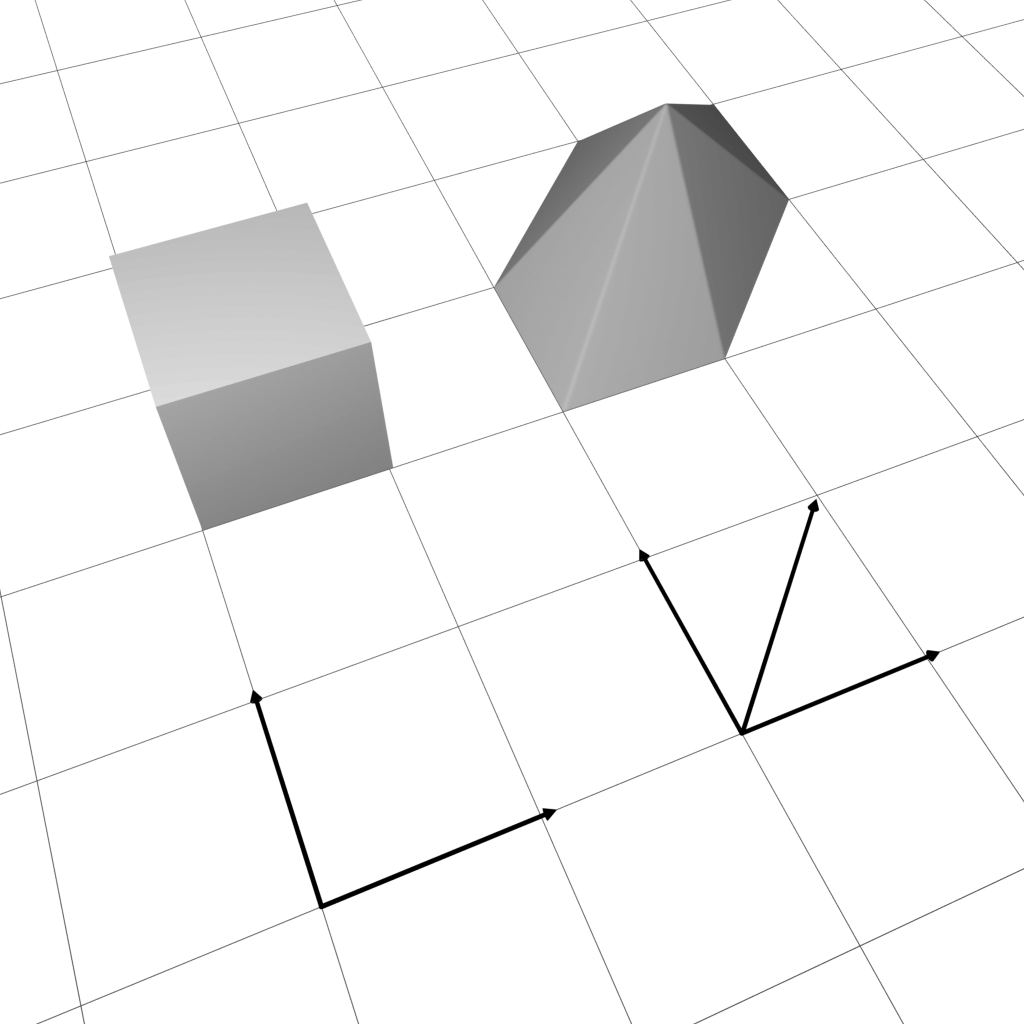
\includegraphics[width=\linewidth]{figures/boxspline/2dex}
  \caption{\label{fig:box2d}%
  An example of box splines in 2D. On the left is the box spline comprised of the direction vectors $\mathbf{\xi}_1, \mathbf{\xi}_2$, (the case n=s) which is the indicator function of the Minkowski sum of the vectors. The box spline on the right, includes a third vector $\mathbf{\xi}_3$, which can be thought of as ``smearing'' the first spline along the direction $\mathbf{\xi}_3$.
  }
\end{figure}


\subsection{Irregular Sampling}
\label{sec:vari_review}
%When reconstructing functions whose data are sampled regularly on a lattice, finding an oblique projection of the original function in the target function space is relatively straight-forward. However, except on very rare occasions, samples placed over the surface of a model do not coincide with lattice sites. A solution to this problem is to ``re-sample'' the input point set onto said lattices sites.
In the work by Kazdhan et al. \cite{fftk} the range data are splatted via a linear filter onto a regular Cartesian grid. This tends to over-smooth the resulting reconstruction, as it allows the surface to deviate from the original sample locations. Ideally, we would like to find a function that not only interpolates the input data, but provides the representation with the smallest possible ``shell'' about the initial point set (i.e., the fewest non zero coefficients) while still interpolating the data and eliciting a unique solution. 

Thus, we recast the problem of finding a representation of $g$ within our function space as an optimization problem. There are similar works that impose variational constraints on random point samples for images \cite{variational}, as well as multi-resolution techniques for volumetric data \cite{onvari} and an extension to box spline spaces \cite{xu2012rec}. In the same vein, we seek a function $g \in \fspce{\varphi}{h\mathbf{L}}$ that attempts to interpolate the input data, and minimize a functional $E$. Specifically, we seek a $g$ that minimizes {\small 
\begin{equation} \label{eq:minexp}
 	\sump_{i=1}^{M} (g(\vx_i) -  f_i)^2 + E(g).
\end{equation}}
It is important to introduce a bit of notation before proceeding, $\dv{\mathbf{v}} f := \mathbf{v} \cdot \grad f$ defines the directional derivative of $f$ in the direction $\mathbf{v}$. The Beppo-Levi inner product of order $n$ is defined as $\blip{n}{f}{g}:= \sum_{|\mathbf{p}|=n}({n!}/{\mathbf{p}!}) \innerp{\mathbf{D^p}f}{\mathbf{D^p}g}$, where $\mathbf{p}$ is an integer vector such that $\left| \mathbf{p}\right| := p_1 + p_2 + p_3 $. We also use the short hand $\mathbf{D^p}f := \partial^{\left| \mathbf{p}\right|}f/({\partial^{p_1}x_1}{\partial^{p_2}x_2}{\partial^{p_3}x_3}).$ The second order Beppo-Levi norm of $f$ is defined as $\bln{2}{f}^2:=\blip{2}{f}{f}$.

The second order Beppo-Levi norm can be thought to measure the ``smoothness'' of a function. However, constraining the smoothness of our approximation alone is not sufficient to elicit the desired solution in our case. We propose that the smoothed normal field should also minimize the inner product of the function with itself. This has the physical interpretation of forcing the solution to be close to zero everywhere except near the input points. Our proposed cost functional is then $E(g) := \lambda_1 \left|\left|{g}\right|\right| + \lambda_2 \bln{2}{g}.$ Here, $\lambda_1$ controls the amount to which the function is penalized for large coefficient values. When combined with the interpolation constraint, this imposes the behavior of forcing the function to be zero away from the surface. The parameter $\lambda_2$ controls the smoothness of the resulting normal field.
%\begin{equation} \label{eq:functional}
%	E(g) := \lambda_1 \left|\left|{g}\right|\right| + \lambda_2 \bln{2}{g}.
%\end{equation}

Finding $g$ that minimizes equation \EQ{eq:minexp} involves rewriting the minimization problem in terms of $\mathbf{c}$ \cite{xu2012rec}. Following some straightforward algebraic manipulations (see \cite{xu2012rec} for details), the coefficient vector can be obtained by taking $\mathbf{c} = ( \mathbf{\Phii}^T\mathbf{\Phii} + \lambda_1\mathbf{G} + \lambda_2\mathbf{S})^{-1}\mathbf{\Phii}^T\mathbf{f}$, where $G_{i,j}:=\innerp{\varphi_i}{\varphi_j}$ and $S_{i,j}:=\blip{2}{\varphi_i}{\varphi_j}$. Since $\varphi$ is known in closed form, the entries of both $\mathbf{G}$ and $\mathbf{S}$ can be evaluated analytically. The above vector equation can be efficiently solved using the Conjugate Gradient method.
%\begin{equation}
%	\mathbf{c} = \left( \mathbf{\Phii}^T\mathbf{\Phii} + \lambda_1\mathbf{G} + \lambda_2\mathbf{S}\right)^{-1}\mathbf{\Phii}^T\mathbf{f},
%\label{eq:variationalSolution}
%\end{equation}

% An example of a floating figure using the graphicx package.
% Note that \label must occur AFTER (or within) \caption.
% For figures, \caption should occur after the \includegraphics.
% Note that IEEEtran v1.7 and later has special internal code that
% is designed to preserve the operation of \label within \caption
% even when the captionsoff option is in effect. However, because
% of issues like this, it may be the safest practice to put all your
% \label just after \caption rather than within \caption{}.
%
% Reminder: the "draftcls" or "draftclsnofoot", not "draft", class
% option should be used if it is desired that the figures are to be
% displayed while in draft mode.
%
%\begin{figure}[!t]
%\centering
%\includegraphics[width=2.5in]{myfigure}
% where an .eps filename suffix will be assumed under latex, 
% and a .pdf suffix will be assumed for pdflatex; or what has been declared
% via \DeclareGraphicsExtensions.
%\caption{Simulation Results}
%\label{fig_sim}
%\end{figure}

% Note that IEEE typically puts floats only at the top, even when this
% results in a large percentage of a column being occupied by floats.


% An example of a double column floating figure using two subfigures.
% (The subfig.sty package must be loaded for this to work.)
% The subfigure \label commands are set within each subfloat command, the
% \label for the overall figure must come after \caption.
% \hfil must be used as a separator to get equal spacing.
% The subfigure.sty package works much the same way, except \subfigure is
% used instead of \subfloat.
%
%\begin{figure*}[!t]
%\centerline{\subfloat[Case I]\includegraphics[width=2.5in]{subfigcase1}%
%\label{fig_first_case}}
%\hfil
%\subfloat[Case II]{\includegraphics[width=2.5in]{subfigcase2}%
%\label{fig_second_case}}}
%\caption{Simulation results}
%\label{fig_sim}
%\end{figure*}
%
% Note that often IEEE papers with subfigures do not employ subfigure
% captions (using the optional argument to \subfloat), but instead will
% reference/describe all of them (a), (b), etc., within the main caption.


% An example of a floating table. Note that, for IEEE style tables, the 
% \caption command should come BEFORE the table. Table text will default to
% \footnotesize as IEEE normally uses this smaller font for tables.
% The \label must come after \caption as always.
%
%\begin{table}[!t]
%% increase table row spacing, adjust to taste
%\renewcommand{\arraystretch}{1.3}
% if using array.sty, it might be a good idea to tweak the value of
% \extrarowheight as needed to properly center the text within the cells
%\caption{An Example of a Table}
%\label{table_example}
%\centering
%% Some packages, such as MDW tools, offer better commands for making tables
%% than the plain LaTeX2e tabular which is used here.
%\begin{tabular}{|c||c|}
%\hline
%One & Two\\
%\hline
%Three & Four\\
%\hline
%\end{tabular}
%\end{table}


% Note that IEEE does not put floats in the very first column - or typically
% anywhere on the first page for that matter. Also, in-text middle ("here")
% positioning is not used. Most IEEE journals use top floats exclusively.
% Note that, LaTeX2e, unlike IEEE journals, places footnotes above bottom
% floats. This can be corrected via the \fnbelowfloat command of the
% stfloats package.



\section{Conclusion}
The conclusion goes here.





% if have a single appendix:
%\appendix[Proof of the Zonklar Equations]
% or
%\appendix  % for no appendix heading
% do not use \section anymore after \appendix, only \section*
% is possibly needed

% use appendices with more than one appendix
% then use \section to start each appendix
% you must declare a \section before using any
% \subsection or using \label (\appendices by itself
% starts a section numbered zero.)
%


\appendices
\section{Proof of the First Zonklar Equation}
Appendix one text goes here.

% you can choose not to have a title for an appendix
% if you want by leaving the argument blank
\section{}
Appendix two text goes here.


% use section* for acknowledgement
\section*{Acknowledgment}


The authors would like to thank...


% Can use something like this to put references on a page
% by themselves when using endfloat and the captionsoff option.
\ifCLASSOPTIONcaptionsoff
  \newpage
\fi



% trigger a \newpage just before the given reference
% number - used to balance the columns on the last page
% adjust value as needed - may need to be readjusted if
% the document is modified later
%\IEEEtriggeratref{8}
% The "triggered" command can be changed if desired:
%\IEEEtriggercmd{\enlargethispage{-5in}}

% references section

% can use a bibliography generated by BibTeX as a .bbl file
% BibTeX documentation can be easily obtained at:
% http://www.ctan.org/tex-archive/biblio/bibtex/contrib/doc/
% The IEEEtran BibTeX style support page is at:
% http://www.michaelshell.org/tex/ieeetran/bibtex/
\bibliographystyle{IEEEtran}
% argument is your BibTeX string definitions and bibliography database(s)
\bibliography{IEEEabrv,./paper.bib}
%
% <OR> manually copy in the resultant .bbl file
% set second argument of \begin to the number of references
% (used to reserve space for the reference number labels box)

%\bibliography{paper}

% biography section
% 
% If you have an EPS/PDF photo (graphicx package needed) extra braces are
% needed around the contents of the optional argument to biography to prevent
% the LaTeX parser from getting confused when it sees the complicated
% \includegraphics command within an optional argument. (You could create
% your own custom macro containing the \includegraphics command to make things
% simpler here.)
%\begin{biography}[{\includegraphics[width=1in,height=1.25in,clip,keepaspectratio]{mshell}}]{Michael Shell}
% or if you just want to reserve a space for a photo:

\begin{IEEEbiography}{Michael Shell}
Biography text here.
\end{IEEEbiography}

% if you will not have a photo at all:
\begin{IEEEbiographynophoto}{John Doe}
Biography text here.
\end{IEEEbiographynophoto}

% insert where needed to balance the two columns on the last page with
% biographies
%\newpage

\begin{IEEEbiographynophoto}{Jane Doe}
Biography text here.
\end{IEEEbiographynophoto}

% You can push biographies down or up by placing
% a \vfill before or after them. The appropriate
% use of \vfill depends on what kind of text is
% on the last page and whether or not the columns
% are being equalized.

%\vfill

% Can be used to pull up biographies so that the bottom of the last one
% is flush with the other column.
%\enlargethispage{-5in}



% that's all folks
\end{document}


